% Options for packages loaded elsewhere
\PassOptionsToPackage{unicode}{hyperref}
\PassOptionsToPackage{hyphens}{url}
%
\documentclass[
]{book}
\usepackage{amsmath,amssymb}
\usepackage{iftex}
\ifPDFTeX
  \usepackage[T1]{fontenc}
  \usepackage[utf8]{inputenc}
  \usepackage{textcomp} % provide euro and other symbols
\else % if luatex or xetex
  \usepackage{unicode-math} % this also loads fontspec
  \defaultfontfeatures{Scale=MatchLowercase}
  \defaultfontfeatures[\rmfamily]{Ligatures=TeX,Scale=1}
\fi
\usepackage{lmodern}
\ifPDFTeX\else
  % xetex/luatex font selection
\fi
% Use upquote if available, for straight quotes in verbatim environments
\IfFileExists{upquote.sty}{\usepackage{upquote}}{}
\IfFileExists{microtype.sty}{% use microtype if available
  \usepackage[]{microtype}
  \UseMicrotypeSet[protrusion]{basicmath} % disable protrusion for tt fonts
}{}
\makeatletter
\@ifundefined{KOMAClassName}{% if non-KOMA class
  \IfFileExists{parskip.sty}{%
    \usepackage{parskip}
  }{% else
    \setlength{\parindent}{0pt}
    \setlength{\parskip}{6pt plus 2pt minus 1pt}}
}{% if KOMA class
  \KOMAoptions{parskip=half}}
\makeatother
\usepackage{xcolor}
\usepackage{color}
\usepackage{fancyvrb}
\newcommand{\VerbBar}{|}
\newcommand{\VERB}{\Verb[commandchars=\\\{\}]}
\DefineVerbatimEnvironment{Highlighting}{Verbatim}{commandchars=\\\{\}}
% Add ',fontsize=\small' for more characters per line
\usepackage{framed}
\definecolor{shadecolor}{RGB}{248,248,248}
\newenvironment{Shaded}{\begin{snugshade}}{\end{snugshade}}
\newcommand{\AlertTok}[1]{\textcolor[rgb]{0.94,0.16,0.16}{#1}}
\newcommand{\AnnotationTok}[1]{\textcolor[rgb]{0.56,0.35,0.01}{\textbf{\textit{#1}}}}
\newcommand{\AttributeTok}[1]{\textcolor[rgb]{0.13,0.29,0.53}{#1}}
\newcommand{\BaseNTok}[1]{\textcolor[rgb]{0.00,0.00,0.81}{#1}}
\newcommand{\BuiltInTok}[1]{#1}
\newcommand{\CharTok}[1]{\textcolor[rgb]{0.31,0.60,0.02}{#1}}
\newcommand{\CommentTok}[1]{\textcolor[rgb]{0.56,0.35,0.01}{\textit{#1}}}
\newcommand{\CommentVarTok}[1]{\textcolor[rgb]{0.56,0.35,0.01}{\textbf{\textit{#1}}}}
\newcommand{\ConstantTok}[1]{\textcolor[rgb]{0.56,0.35,0.01}{#1}}
\newcommand{\ControlFlowTok}[1]{\textcolor[rgb]{0.13,0.29,0.53}{\textbf{#1}}}
\newcommand{\DataTypeTok}[1]{\textcolor[rgb]{0.13,0.29,0.53}{#1}}
\newcommand{\DecValTok}[1]{\textcolor[rgb]{0.00,0.00,0.81}{#1}}
\newcommand{\DocumentationTok}[1]{\textcolor[rgb]{0.56,0.35,0.01}{\textbf{\textit{#1}}}}
\newcommand{\ErrorTok}[1]{\textcolor[rgb]{0.64,0.00,0.00}{\textbf{#1}}}
\newcommand{\ExtensionTok}[1]{#1}
\newcommand{\FloatTok}[1]{\textcolor[rgb]{0.00,0.00,0.81}{#1}}
\newcommand{\FunctionTok}[1]{\textcolor[rgb]{0.13,0.29,0.53}{\textbf{#1}}}
\newcommand{\ImportTok}[1]{#1}
\newcommand{\InformationTok}[1]{\textcolor[rgb]{0.56,0.35,0.01}{\textbf{\textit{#1}}}}
\newcommand{\KeywordTok}[1]{\textcolor[rgb]{0.13,0.29,0.53}{\textbf{#1}}}
\newcommand{\NormalTok}[1]{#1}
\newcommand{\OperatorTok}[1]{\textcolor[rgb]{0.81,0.36,0.00}{\textbf{#1}}}
\newcommand{\OtherTok}[1]{\textcolor[rgb]{0.56,0.35,0.01}{#1}}
\newcommand{\PreprocessorTok}[1]{\textcolor[rgb]{0.56,0.35,0.01}{\textit{#1}}}
\newcommand{\RegionMarkerTok}[1]{#1}
\newcommand{\SpecialCharTok}[1]{\textcolor[rgb]{0.81,0.36,0.00}{\textbf{#1}}}
\newcommand{\SpecialStringTok}[1]{\textcolor[rgb]{0.31,0.60,0.02}{#1}}
\newcommand{\StringTok}[1]{\textcolor[rgb]{0.31,0.60,0.02}{#1}}
\newcommand{\VariableTok}[1]{\textcolor[rgb]{0.00,0.00,0.00}{#1}}
\newcommand{\VerbatimStringTok}[1]{\textcolor[rgb]{0.31,0.60,0.02}{#1}}
\newcommand{\WarningTok}[1]{\textcolor[rgb]{0.56,0.35,0.01}{\textbf{\textit{#1}}}}
\usepackage{longtable,booktabs,array}
\usepackage{calc} % for calculating minipage widths
% Correct order of tables after \paragraph or \subparagraph
\usepackage{etoolbox}
\makeatletter
\patchcmd\longtable{\par}{\if@noskipsec\mbox{}\fi\par}{}{}
\makeatother
% Allow footnotes in longtable head/foot
\IfFileExists{footnotehyper.sty}{\usepackage{footnotehyper}}{\usepackage{footnote}}
\makesavenoteenv{longtable}
\usepackage{graphicx}
\makeatletter
\newsavebox\pandoc@box
\newcommand*\pandocbounded[1]{% scales image to fit in text height/width
  \sbox\pandoc@box{#1}%
  \Gscale@div\@tempa{\textheight}{\dimexpr\ht\pandoc@box+\dp\pandoc@box\relax}%
  \Gscale@div\@tempb{\linewidth}{\wd\pandoc@box}%
  \ifdim\@tempb\p@<\@tempa\p@\let\@tempa\@tempb\fi% select the smaller of both
  \ifdim\@tempa\p@<\p@\scalebox{\@tempa}{\usebox\pandoc@box}%
  \else\usebox{\pandoc@box}%
  \fi%
}
% Set default figure placement to htbp
\def\fps@figure{htbp}
\makeatother
\setlength{\emergencystretch}{3em} % prevent overfull lines
\providecommand{\tightlist}{%
  \setlength{\itemsep}{0pt}\setlength{\parskip}{0pt}}
\setcounter{secnumdepth}{5}
\usepackage{booktabs}
\usepackage[]{natbib}
\bibliographystyle{apa}
\nocite{ram_tethering_2012, revelle_psych_2024, wickham_dplyr_2023, wickham_tidyr_2024, wickham_ggplot2_2016, wickham_welcome_2019}
\usepackage{bookmark}
\IfFileExists{xurl.sty}{\usepackage{xurl}}{} % add URL line breaks if available
\urlstyle{same}
\hypersetup{
  pdftitle={Intensive Longitudinal Analysis},
  pdfauthor={Kevin Grimm, Nilam Ram et. al.},
  hidelinks,
  pdfcreator={LaTeX via pandoc}}

\title{Intensive Longitudinal Analysis}
\author{Kevin Grimm, Nilam Ram et. al.}
\date{2025-08-14}

\usepackage{amsthm}
\newtheorem{theorem}{Theorem}[chapter]
\newtheorem{lemma}{Lemma}[chapter]
\newtheorem{corollary}{Corollary}[chapter]
\newtheorem{proposition}{Proposition}[chapter]
\newtheorem{conjecture}{Conjecture}[chapter]
\theoremstyle{definition}
\newtheorem{definition}{Definition}[chapter]
\theoremstyle{definition}
\newtheorem{example}{Example}[chapter]
\theoremstyle{definition}
\newtheorem{exercise}{Exercise}[chapter]
\theoremstyle{definition}
\newtheorem{hypothesis}{Hypothesis}[chapter]
\theoremstyle{remark}
\newtheorem*{remark}{Remark}
\newtheorem*{solution}{Solution}
\begin{document}
\maketitle

{
\setcounter{tocdepth}{1}
\tableofcontents
}
\chapter{Intensive Longitudinal Data \& Analysis}\label{intensive-longitudinal-data-analysis}

\section{Chapters}\label{chapters}

\hyperref[amib]{AMIB}

\hyperref[data-descriptives-dataviz]{Data Descriptives and Data Viz}

Chapter \ref{amib} ``AMIB''

Chapter \ref{data-descriptives-dataviz} ``Data Descriptives and Data
Viz''

\section{Let's Try A Picture!}\label{lets-try-a-picture}

\href{https://www.youtube.com/watch?v=dQw4w9WgXcQ}{\pandocbounded{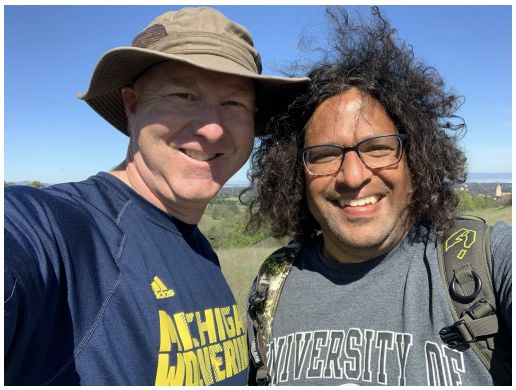
\includegraphics[keepaspectratio]{Kevin_Nilam.png}}}

\section{Fun Quotes}\label{fun-quotes}

\begin{quote}
``\ldots{} ideal longitudinal research is characterized by the seamless
integration of a well-articulated theoretical model of change, an
appropriate temporal design, and a statistical model that is an
operationalization of the theoretical model.''
\citet{collins_analysis_2006}
\end{quote}

\begin{quote}
``Longitudinal methodology involves repeated, time- ordered observation
of an {[}entity{]} or {[}entities{]} with the goal of identifying processes
and causes \ldots{}'' \citet{nesselroade_longitudinal_1979}
\end{quote}

\begin{quote}
``Intensive longitudinal methods involve sequences of repeated
measurements sufficiently frequent to allow one to characterize
{[}functional form of change + causes and consequences{]} a separate
change process for each subject (which can be a person or other
sampling unit such as dyad or group).''
\end{quote}

\begin{itemize}
\item
  Experience sampling, daily diaries, interaction records, ecological
  momentary assessment, ambulatory assessment, real-time data capture

  \begin{itemize}
  \tightlist
  \item
    Justifications: ``life as it is lived'', non-ergodicity
    (description of within-person processes)
  \end{itemize}
\end{itemize}

\section{Intensive Longitudinal Studies}\label{intensive-longitudinal-studies}

\begin{itemize}
\item
  An intensive longitudinal study is one with enough repeated
  measurements to model a distinct change process for each individual
  •

  \begin{itemize}
  \item
    Within-individual variability is key
  \item
    Time scale: minutes, hours, days, and weeks rather than months
    and years
  \item
    Used to understand people's thoughts, feelings, and behaviors as
    it happens
  \end{itemize}
\end{itemize}

\section{Information About}\label{information-about}

This is a \emph{sample} book written in \textbf{Markdown}. You can use anything
that Pandoc's Markdown supports; for example, a math equation
\(a^2 + b^2 = c^2\).

\chapter{AMIB}\label{amib}

Our examples make use of \href{https://thechangelab.stanford.edu/collaborations/the-amib-data/}{\textbf{The AMIB Data}}, a multiple time-scale data set that has been shared for teaching purposes.
The data include person-level \emph{dispositions}, \emph{daily} diary assessments, and ecological momentary assessments that were obtained after everyday social \emph{interactions} (event-contingent sampling).

The data are shared with intent to facilitate learning about analysis of \emph{intensive longitudinal data} (from experience sampling, daily diary, or EMA designs).
\textbf{The data are posted only for teaching purposes and should not be used for research.}

Use requires citation and acknowledgement of both this website and the following paper:

Ram, N., Conroy, D. E., Pincus, A. L., Hyde, A. L., \& Molloy, L. E. (2012). Tethering theory to method: Using measures of intraindividual variability to operationalize individuals' dynamic characteristics. In G. Hancock \& J. Harring (Eds.), \emph{Advances in longitudinal methods in the social and behavioral sciences} (pp.~81-110). New York: Information Age.\\

\chapter{Data, Descriptives \& Data Viz}\label{data-descriptives-dataviz}

This tutorial walks through a few helpful initial steps before analysis of experience sampling and EMA data (or any analyses, actually).

\section{Outline}\label{outline}

This chapter covers \ldots{}

A. Loading the AMIB data

B. Describing some aspects of the data

C. A few data visualizations

\subsection{Loading Libraries Used in this Script}\label{loading-libraries-used-in-this-script}

\begin{Shaded}
\begin{Highlighting}[]
\FunctionTok{library}\NormalTok{(psych)      }\CommentTok{\#describing the data}
\FunctionTok{library}\NormalTok{(tidyr)      }\CommentTok{\#tidy data}
\FunctionTok{library}\NormalTok{(dplyr)      }\CommentTok{\#data manipulation}
\FunctionTok{library}\NormalTok{(ggplot2)    }\CommentTok{\#data visualization}

\CommentTok{\#you can load tidyverse (dplyr, forcats, ggplot2, lubridate, purr, rear, stringr, tibble, tidyr) via:}
\CommentTok{\#library(tidyverse)}
\CommentTok{\#we do this in lots of our tutorials and in our own work!}
\end{Highlighting}
\end{Shaded}

\textbf{If you have issues installing the psych package - try installing the psych package again without compilation}

\section{Loading The AMIB Data}\label{loading-the-amib-data}

The first step, and often the most frustrating part of data analysis is\ldots getting the data into the program!

In recent years people are generally exchanging data files in a .csv format as these files port well and can interface with many different software packages.

Here, we make use of the person-level and interaction-level (EMA-type) AMIB data files, which can be merged easily using the \texttt{id} and \texttt{day} variables.

\subsection{\texorpdfstring{Loading person-level file (\emph{N} = 190)}{Loading person-level file (N = 190)}}\label{loading-person-level-file-n-190}

\begin{Shaded}
\begin{Highlighting}[]
\CommentTok{\#set filepath for data file}
\NormalTok{filepath }\OtherTok{\textless{}{-}} \StringTok{"https://raw.githubusercontent.com/The{-}Change{-}Lab/collaborations/main/AMIB/AMIB\_persons.csv"}
\CommentTok{\#read in the .csv file using the url() function}
\NormalTok{AMIB\_persons }\OtherTok{\textless{}{-}} \FunctionTok{read.csv}\NormalTok{(}\AttributeTok{file=}\FunctionTok{url}\NormalTok{(filepath), }\AttributeTok{header=}\ConstantTok{TRUE}\NormalTok{)}
\end{Highlighting}
\end{Shaded}

\subsection{\texorpdfstring{Loading interaction-level file (\emph{T} = many, on average 43 per person)}{Loading interaction-level file (T = many, on average 43 per person)}}\label{loading-interaction-level-file-t-many-on-average-43-per-person}

\begin{Shaded}
\begin{Highlighting}[]
\CommentTok{\#set filepath for data file}
\NormalTok{filepath }\OtherTok{\textless{}{-}} \StringTok{"https://raw.githubusercontent.com/The{-}Change{-}Lab/collaborations/main/AMIB/AMIB\_interaction.csv"}
\CommentTok{\#read in the .csv file using the url() function}
\NormalTok{AMIB\_interaction }\OtherTok{\textless{}{-}} \FunctionTok{read.csv}\NormalTok{(}\AttributeTok{file=}\FunctionTok{url}\NormalTok{(filepath), }\AttributeTok{header=}\ConstantTok{TRUE}\NormalTok{)}
\end{Highlighting}
\end{Shaded}

\section{Describing The AMIB Data}\label{describing-the-amib-data}

Once the data are in, we can begin learning about them.

\subsection{Basic descriptives of person-level data}\label{basic-descriptives-of-person-level-data}

\subsubsection{Subsetting to a few variables}\label{subsetting-to-a-few-variables}

\begin{Shaded}
\begin{Highlighting}[]
\CommentTok{\#subsetting to a few trait variables}
\NormalTok{AMIB\_persons }\OtherTok{\textless{}{-}}\NormalTok{ AMIB\_persons }\SpecialCharTok{\%\textgreater{}\%}
  \FunctionTok{select}\NormalTok{(id, sex, bfi\_o, bfi\_c, bfi\_e, bfi\_a, bfi\_n)}
\CommentTok{\#note, subsetting with the same name will override the original data that you loaded, and you\textquotesingle{}ll loose the variables you don\textquotesingle{}t select}
\CommentTok{\#if you don\textquotesingle{}t want to loose those variables, subset to a new data frame, ie: AMIB\_persons\_sub \textless{}{-} AMIB\_persons}
\end{Highlighting}
\end{Shaded}

\subsection{Descriptives of traits using person-level data (sex, personality)}\label{descriptives-of-traits-using-person-level-data-sex-personality}

\begin{Shaded}
\begin{Highlighting}[]
\CommentTok{\#basic descriptives (using describe() from the psych package)}
\NormalTok{psych}\SpecialCharTok{::}\FunctionTok{describe}\NormalTok{(AMIB\_persons)}
\CommentTok{\#\textgreater{}       vars   n   mean     sd median trimmed    mad   min}
\CommentTok{\#\textgreater{} id       1 190 318.29 130.44  321.5  318.99 151.23 101.0}
\CommentTok{\#\textgreater{} sex      2 190   1.66   0.48    2.0    1.70   0.00   1.0}
\CommentTok{\#\textgreater{} bfi\_o    3 190   3.60   0.96    3.5    3.64   0.74   1.0}
\CommentTok{\#\textgreater{} bfi\_c    4 190   3.76   0.85    4.0    3.77   0.74   1.5}
\CommentTok{\#\textgreater{} bfi\_e    5 190   3.38   1.00    3.5    3.40   0.74   1.0}
\CommentTok{\#\textgreater{} bfi\_a    6 190   3.61   0.88    3.5    3.69   0.74   1.0}
\CommentTok{\#\textgreater{} bfi\_n    7 190   2.98   0.96    3.0    3.00   1.48   1.0}
\CommentTok{\#\textgreater{}       max range  skew kurtosis   se}
\CommentTok{\#\textgreater{} id    532 431.0 {-}0.04    {-}1.09 9.46}
\CommentTok{\#\textgreater{} sex     2   1.0 {-}0.66    {-}1.57 0.03}
\CommentTok{\#\textgreater{} bfi\_o   5   4.0 {-}0.34    {-}0.48 0.07}
\CommentTok{\#\textgreater{} bfi\_c   5   3.5 {-}0.12    {-}0.90 0.06}
\CommentTok{\#\textgreater{} bfi\_e   5   4.0 {-}0.21    {-}0.58 0.07}
\CommentTok{\#\textgreater{} bfi\_a   5   4.0 {-}0.72     0.14 0.06}
\CommentTok{\#\textgreater{} bfi\_n   5   4.0 {-}0.09    {-}0.82 0.07}
\CommentTok{\#note: some psych and dplyr functions overlap. You have to specify your package by package::function(data)}

\CommentTok{\#correlations}
\FunctionTok{cor}\NormalTok{(AMIB\_persons[ ,}\SpecialCharTok{{-}}\DecValTok{1}\NormalTok{]) }\CommentTok{\#dropping 1st column (id)}
\CommentTok{\#\textgreater{}              sex       bfi\_o       bfi\_c       bfi\_e}
\CommentTok{\#\textgreater{} sex   1.00000000  0.06161000  0.03394367  0.18873546}
\CommentTok{\#\textgreater{} bfi\_o 0.06161000  1.00000000  0.03093131  0.13087435}
\CommentTok{\#\textgreater{} bfi\_c 0.03394367  0.03093131  1.00000000 {-}0.01870259}
\CommentTok{\#\textgreater{} bfi\_e 0.18873546  0.13087435 {-}0.01870259  1.00000000}
\CommentTok{\#\textgreater{} bfi\_a 0.04422936  0.03581446  0.08472053  0.08558411}
\CommentTok{\#\textgreater{} bfi\_n 0.18389358 {-}0.05557229 {-}0.02838956 {-}0.16160302}
\CommentTok{\#\textgreater{}             bfi\_a       bfi\_n}
\CommentTok{\#\textgreater{} sex    0.04422936  0.18389358}
\CommentTok{\#\textgreater{} bfi\_o  0.03581446 {-}0.05557229}
\CommentTok{\#\textgreater{} bfi\_c  0.08472053 {-}0.02838956}
\CommentTok{\#\textgreater{} bfi\_e  0.08558411 {-}0.16160302}
\CommentTok{\#\textgreater{} bfi\_a  1.00000000 {-}0.12293379}
\CommentTok{\#\textgreater{} bfi\_n {-}0.12293379  1.00000000}

\CommentTok{\#plot matrix (usingpairs.panels from the psych package)}
\NormalTok{psych}\SpecialCharTok{::}\FunctionTok{pairs.panels}\NormalTok{(AMIB\_persons[ ,}\SpecialCharTok{{-}}\DecValTok{1}\NormalTok{])}
\end{Highlighting}
\end{Shaded}

\pandocbounded{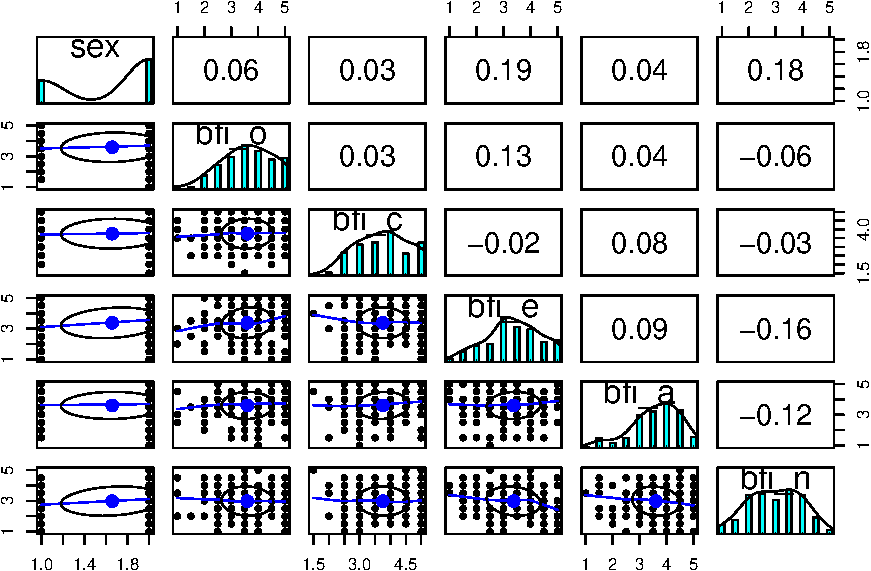
\includegraphics[keepaspectratio]{02_data-descriptives-dataviz_files/figure-latex/describe-1.pdf}}

Note that the person-level descriptives are ``cross-sectional''.

\subsection{Basic descriptives of interaction-level data}\label{basic-descriptives-of-interaction-level-data}

Subsetting to a few variables:

\begin{itemize}
\item
  ID and TIME variables: \texttt{id}, \texttt{day}, \texttt{interaction}, \texttt{timea}
\item
  Outcome variables: \texttt{partner\_gender}, \texttt{agval}, \texttt{stress}
\end{itemize}

\begin{Shaded}
\begin{Highlighting}[]
\CommentTok{\#subsetting to a few variables}
\NormalTok{AMIB\_interaction }\OtherTok{\textless{}{-}}\NormalTok{ AMIB\_interaction }\SpecialCharTok{\%\textgreater{}\%}
  \FunctionTok{select}\NormalTok{(id, day, interaction, timea, partner\_gender, agval, stress)}
\end{Highlighting}
\end{Shaded}

Often, our analyses will make use of both the repeated measures data and the person-level data.
For illustration, we merge them here.

\subsection{Merging person-level data into repeated measures interaction-level data}\label{merging-person-level-data-into-repeated-measures-interaction-level-data}

\begin{Shaded}
\begin{Highlighting}[]
\CommentTok{\#merging repeated measures and person{-}level data}
\NormalTok{interaction\_long }\OtherTok{\textless{}{-}}\NormalTok{ AMIB\_interaction }\SpecialCharTok{\%\textgreater{}\%}
  \FunctionTok{left\_join}\NormalTok{(AMIB\_persons, }\AttributeTok{by=}\StringTok{"id"}\NormalTok{)}

\CommentTok{\#look at first few rows of data}
\FunctionTok{head}\NormalTok{(interaction\_long, }\DecValTok{10}\NormalTok{)}
\CommentTok{\#\textgreater{}     id day interaction timea partner\_gender agval stress}
\CommentTok{\#\textgreater{} 1  101   1           1   700              0     3      1}
\CommentTok{\#\textgreater{} 2  101   1           2  1230              1     8      1}
\CommentTok{\#\textgreater{} 3  101   1           3  1245              1     8      1}
\CommentTok{\#\textgreater{} 4  101   1           4  1330              1     8      1}
\CommentTok{\#\textgreater{} 5  101   1           5  1420              1     6      1}
\CommentTok{\#\textgreater{} 6  101   1           6  1445              1     8      1}
\CommentTok{\#\textgreater{} 7  101   1           7  1920              1     8      1}
\CommentTok{\#\textgreater{} 8  101   1           8  2030              1     8      1}
\CommentTok{\#\textgreater{} 9  101   2           9    30              0     9      0}
\CommentTok{\#\textgreater{} 10 101   2          10     0              1     8      0}
\CommentTok{\#\textgreater{}    sex bfi\_o bfi\_c bfi\_e bfi\_a bfi\_n}
\CommentTok{\#\textgreater{} 1    2     4     4   3.5   1.5     2}
\CommentTok{\#\textgreater{} 2    2     4     4   3.5   1.5     2}
\CommentTok{\#\textgreater{} 3    2     4     4   3.5   1.5     2}
\CommentTok{\#\textgreater{} 4    2     4     4   3.5   1.5     2}
\CommentTok{\#\textgreater{} 5    2     4     4   3.5   1.5     2}
\CommentTok{\#\textgreater{} 6    2     4     4   3.5   1.5     2}
\CommentTok{\#\textgreater{} 7    2     4     4   3.5   1.5     2}
\CommentTok{\#\textgreater{} 8    2     4     4   3.5   1.5     2}
\CommentTok{\#\textgreater{} 9    2     4     4   3.5   1.5     2}
\CommentTok{\#\textgreater{} 10   2     4     4   3.5   1.5     2}

\CommentTok{\#checking number of persons}
\FunctionTok{length}\NormalTok{(}\FunctionTok{unique}\NormalTok{(interaction\_long}\SpecialCharTok{$}\NormalTok{id))}
\CommentTok{\#\textgreater{} [1] 184}
\end{Highlighting}
\end{Shaded}

Note that there are only 184 persons in the data now (vs.~\emph{N} = 190 in the person-level file).

In this case, the discrepancy is because there were 6 persons that completed baseline questionnaires, but did not provide any EMA data.

\subsection{Descriptives of the merged interaction-level and person-level data}\label{descriptives-of-the-merged-interaction-level-and-person-level-data}

\begin{Shaded}
\begin{Highlighting}[]
\CommentTok{\#basic descriptives}
\NormalTok{psych}\SpecialCharTok{::}\FunctionTok{describe}\NormalTok{(interaction\_long)}
\CommentTok{\#\textgreater{}                vars    n    mean     sd median trimmed}
\CommentTok{\#\textgreater{} id                1 7568  330.55 122.47  328.0  334.09}
\CommentTok{\#\textgreater{} day               2 7568    3.97   1.99    4.0    3.96}
\CommentTok{\#\textgreater{} interaction       3 7568   23.31  14.74   22.0   22.56}
\CommentTok{\#\textgreater{} timea             4 7500 1496.82 445.29 1500.0 1495.34}
\CommentTok{\#\textgreater{} partner\_gender    5 6884    0.60   0.49    1.0    0.62}
\CommentTok{\#\textgreater{} agval             6 7553    6.68   1.96    7.0    6.92}
\CommentTok{\#\textgreater{} stress            7 7544    1.31   1.33    1.0    1.14}
\CommentTok{\#\textgreater{} sex               8 7568    1.70   0.46    2.0    1.75}
\CommentTok{\#\textgreater{} bfi\_o             9 7568    3.60   0.95    3.5    3.64}
\CommentTok{\#\textgreater{} bfi\_c            10 7568    3.77   0.85    4.0    3.79}
\CommentTok{\#\textgreater{} bfi\_e            11 7568    3.41   0.97    3.5    3.43}
\CommentTok{\#\textgreater{} bfi\_a            12 7568    3.61   0.87    3.5    3.69}
\CommentTok{\#\textgreater{} bfi\_n            13 7568    3.00   0.96    3.0    3.00}
\CommentTok{\#\textgreater{}                   mad   min  max  range  skew kurtosis   se}
\CommentTok{\#\textgreater{} id             145.29 101.0  532  431.0 {-}0.17    {-}0.91 1.41}
\CommentTok{\#\textgreater{} day              2.97   1.0    7    6.0  0.02    {-}1.24 0.02}
\CommentTok{\#\textgreater{} interaction     17.79   1.0   56   55.0  0.35    {-}0.90 0.17}
\CommentTok{\#\textgreater{} timea          489.26   0.0 2800 2800.0 {-}0.10    {-}0.14 5.14}
\CommentTok{\#\textgreater{} partner\_gender   0.00   0.0    1    1.0 {-}0.39    {-}1.85 0.01}
\CommentTok{\#\textgreater{} agval            1.48   1.0    9    8.0 {-}0.95     0.33 0.02}
\CommentTok{\#\textgreater{} stress           1.48   0.0    5    5.0  0.77    {-}0.32 0.02}
\CommentTok{\#\textgreater{} sex              0.00   1.0    2    1.0 {-}0.85    {-}1.27 0.01}
\CommentTok{\#\textgreater{} bfi\_o            0.74   1.0    5    4.0 {-}0.41    {-}0.24 0.01}
\CommentTok{\#\textgreater{} bfi\_c            0.74   1.5    5    3.5 {-}0.15    {-}0.86 0.01}
\CommentTok{\#\textgreater{} bfi\_e            0.74   1.0    5    4.0 {-}0.24    {-}0.52 0.01}
\CommentTok{\#\textgreater{} bfi\_a            0.74   1.0    5    4.0 {-}0.65    {-}0.02 0.01}
\CommentTok{\#\textgreater{} bfi\_n            1.48   1.0    5    4.0 {-}0.03    {-}0.76 0.01}

\CommentTok{\#plot matrix}
\NormalTok{psych}\SpecialCharTok{::}\FunctionTok{pairs.panels}\NormalTok{(interaction\_long[ ,}\FunctionTok{c}\NormalTok{(}\StringTok{"partner\_gender"}\NormalTok{,}\StringTok{"agval"}\NormalTok{,}\StringTok{"stress"}\NormalTok{)])}
\end{Highlighting}
\end{Shaded}

\pandocbounded{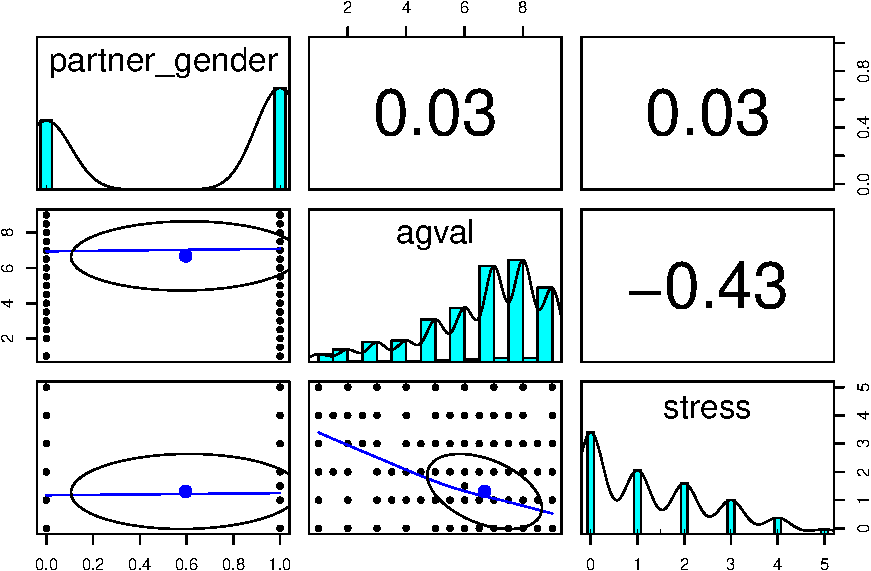
\includegraphics[keepaspectratio]{02_data-descriptives-dataviz_files/figure-latex/descrbe merged-1.pdf}}

\textbf{BE CAREFUL!}

These descriptives ignore the nesting of the data (i.e., they are a mix of within-person and between-person information).

\subsection{Describing compliance (and missing data)}\label{describing-compliance-and-missing-data}

Among the first steps when describing experience sampling data is describing the number of observations.
\emph{The protocol was designed for 8 reports per day for 7 days = 56 observations maximum per person.}

\begin{Shaded}
\begin{Highlighting}[]
\CommentTok{\# counts of days (day 0 to day 8) completed}
\FunctionTok{table}\NormalTok{(interaction\_long}\SpecialCharTok{$}\NormalTok{day)}
\CommentTok{\#\textgreater{} }
\CommentTok{\#\textgreater{}    1    2    3    4    5    6    7 }
\CommentTok{\#\textgreater{} 1101 1094 1071 1128 1055 1076 1043}

\CommentTok{\#counting number of days and interaction reports completed for each person}
\NormalTok{compliance\_stats }\OtherTok{\textless{}{-}}\NormalTok{ interaction\_long }\SpecialCharTok{\%\textgreater{}\%}
  \FunctionTok{group\_by}\NormalTok{(id) }\SpecialCharTok{\%\textgreater{}\%}   \CommentTok{\#specify the unit we want to summarise by, in this case per person}
  \FunctionTok{summarise}\NormalTok{(}\AttributeTok{num\_days =} \FunctionTok{length}\NormalTok{(}\FunctionTok{unique}\NormalTok{(day)),}
            \AttributeTok{num\_obs =} \FunctionTok{length}\NormalTok{(id))}

\CommentTok{\# looking at counts}
\FunctionTok{describe}\NormalTok{(compliance\_stats)}
\CommentTok{\#\textgreater{}          vars   n   mean     sd median trimmed    mad min}
\CommentTok{\#\textgreater{} id          1 184 321.97 129.72  323.5  323.39 151.23 101}
\CommentTok{\#\textgreater{} num\_days    2 184   6.82   0.64    7.0    6.99   0.00   2}
\CommentTok{\#\textgreater{} num\_obs     3 184  41.13  13.62   43.0   42.45  17.79  10}
\CommentTok{\#\textgreater{}          max range  skew kurtosis   se}
\CommentTok{\#\textgreater{} id       532   431 {-}0.07    {-}1.09 9.56}
\CommentTok{\#\textgreater{} num\_days   7     5 {-}4.66    25.30 0.05}
\CommentTok{\#\textgreater{} num\_obs   56    46 {-}0.53    {-}0.94 1.00}
\FunctionTok{table}\NormalTok{(compliance\_stats}\SpecialCharTok{$}\NormalTok{num\_days, }\AttributeTok{useNA =} \StringTok{"always"}\NormalTok{)}
\CommentTok{\#\textgreater{} }
\CommentTok{\#\textgreater{}    2    3    4    5    6    7 \textless{}NA\textgreater{} }
\CommentTok{\#\textgreater{}    1    1    1    5   11  165    0}
\FunctionTok{table}\NormalTok{(compliance\_stats}\SpecialCharTok{$}\NormalTok{num\_obs, }\AttributeTok{useNA =} \StringTok{"always"}\NormalTok{)}
\CommentTok{\#\textgreater{} }
\CommentTok{\#\textgreater{}   10   11   13   14   15   16   17   18   19   20   22   23 }
\CommentTok{\#\textgreater{}    2    1    1    2    2    3    1    4    2    2    1    5 }
\CommentTok{\#\textgreater{}   25   26   28   29   30   31   32   33   34   35   36   37 }
\CommentTok{\#\textgreater{}    5    2    4    4    4    6    2    4    6    3    3    2 }
\CommentTok{\#\textgreater{}   38   39   40   41   42   43   44   45   46   47   48   49 }
\CommentTok{\#\textgreater{}    1    2    3    5    5    6    2    4    3    4    6    2 }
\CommentTok{\#\textgreater{}   50   51   52   53   54   55   56 \textless{}NA\textgreater{} }
\CommentTok{\#\textgreater{}    5    6    4    2    2    7   44    0}

\CommentTok{\#histogram}
\NormalTok{compliance\_stats }\SpecialCharTok{\%\textgreater{}\%}
  \FunctionTok{ggplot}\NormalTok{(}\FunctionTok{aes}\NormalTok{(}\AttributeTok{x =}\NormalTok{ num\_obs)) }\SpecialCharTok{+}
  \FunctionTok{geom\_histogram}\NormalTok{(}\AttributeTok{fill=}\StringTok{"white"}\NormalTok{, }\AttributeTok{color=}\StringTok{"black"}\NormalTok{) }\SpecialCharTok{+} 
  \FunctionTok{labs}\NormalTok{(}\AttributeTok{x =} \StringTok{"Number of Observations Completed"}\NormalTok{)}
\end{Highlighting}
\end{Shaded}

\pandocbounded{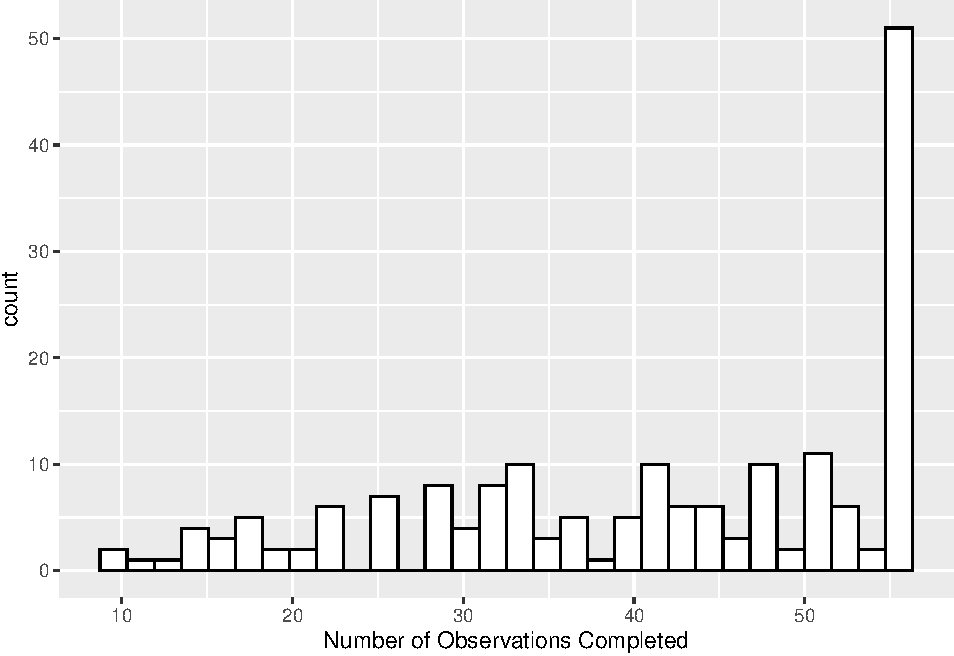
\includegraphics[keepaspectratio]{02_data-descriptives-dataviz_files/figure-latex/compliance-1.pdf}}

Note that the specific way one does these counts depends on the structure of the initial data file - e.g., whether missed reports included or not (here they were not).
The counts can then be summarized for inclusion in a report.

\subsection{Long and Wide Format Data}\label{long-and-wide-format-data}

Behavioral science tends to use relational data structures - i.e., spreadsheets.
Typically the data are stored/configured as a data frame (a ``fancy'' matrix) with multiple rows and multiple columns.

Two main schema are used to accommodate repeated measures data: ``Wide Format'' and ``Long Format''.

Different functions work with different kinds of data formats.
Thus, it is imperative that one can convert the data back and forth between wide and long formats.

\subsubsection{\texorpdfstring{Reshape the data from \textbf{\emph{Long}} to \textbf{\emph{Wide}}}{Reshape the data from Long to Wide}}\label{reshape-the-data-from-long-to-wide}

There are lots of ways to go from long to wide or wide to long.

With the popularity of tidyverse, \texttt{pivot\_wider} and \texttt{pivot\_longer} are taking over for reshaping.
Tidyverse has a good guide for \texttt{pivot\_wider} \href{https://tidyr.tidyverse.org/reference/pivot_wider.html}{here} and for \texttt{pivot\_longer} \href{https://tidyr.tidyverse.org/reference/pivot_longer.html}{here}.

Older popular functions include the \texttt{reshape()} function (not to be confused with the reshape2 package) and \texttt{melt()} and \texttt{cast()} functions in the reshape2 package.

\begin{Shaded}
\begin{Highlighting}[]
\CommentTok{\#trick to get variable names for easy cut{-}and{-}paste}
\FunctionTok{dput}\NormalTok{(}\FunctionTok{names}\NormalTok{(interaction\_long))}
\CommentTok{\#\textgreater{} c("id", "day", "interaction", "timea", "partner\_gender", "agval", }
\CommentTok{\#\textgreater{} "stress", "sex", "bfi\_o", "bfi\_c", "bfi\_e", "bfi\_a", "bfi\_n")}

\CommentTok{\#reshaping long to wide (using tidyr package)}
\NormalTok{interaction\_wide }\OtherTok{\textless{}{-}}\NormalTok{interaction\_long }\SpecialCharTok{\%\textgreater{}\%}
  \FunctionTok{select}\NormalTok{(}\SpecialCharTok{{-}}\NormalTok{day) }\SpecialCharTok{\%\textgreater{}\%} \CommentTok{\#dropping variables not needed}
  \FunctionTok{rename}\NormalTok{(}\AttributeTok{partnergender =}\NormalTok{ partner\_gender) }\SpecialCharTok{\%\textgreater{}\%} \CommentTok{\#renaming to make reshaping easier later}
  \FunctionTok{pivot\_wider}\NormalTok{(}\AttributeTok{id\_cols =} \FunctionTok{c}\NormalTok{(id, sex, bfi\_o, bfi\_c, bfi\_e, bfi\_a, bfi\_n), }\CommentTok{\#column(s) to keep as is}
              \AttributeTok{names\_from =}\NormalTok{ interaction, }\CommentTok{\#column(s) by which to pivot}
              \AttributeTok{values\_from =} \FunctionTok{c}\NormalTok{(timea, partnergender, agval, stress), }\CommentTok{\#column(s) that you want to pivot wider}
              \AttributeTok{names\_sep =} \StringTok{"\_"}\NormalTok{)}

\CommentTok{\#looking at part of data file}
\FunctionTok{head}\NormalTok{(interaction\_wide[,}\DecValTok{1}\SpecialCharTok{:}\DecValTok{10}\NormalTok{], }\DecValTok{10}\NormalTok{)}
\CommentTok{\#\textgreater{} \# A tibble: 10 x 10}
\CommentTok{\#\textgreater{}       id   sex bfi\_o bfi\_c bfi\_e bfi\_a bfi\_n timea\_1 timea\_2}
\CommentTok{\#\textgreater{}    \textless{}int\textgreater{} \textless{}int\textgreater{} \textless{}dbl\textgreater{} \textless{}dbl\textgreater{} \textless{}dbl\textgreater{} \textless{}dbl\textgreater{} \textless{}dbl\textgreater{}   \textless{}int\textgreater{}   \textless{}int\textgreater{}}
\CommentTok{\#\textgreater{}  1   101     2   4     4     3.5   1.5   2       700    1230}
\CommentTok{\#\textgreater{}  2   103     2   5     3.5   4     4.5   2.5    1100    1400}
\CommentTok{\#\textgreater{}  3   104     2   3     4.5   3     4.5   2.5     700     530}
\CommentTok{\#\textgreater{}  4   105     2   4.5   3     3.5   3.5   3.5    1100    1210}
\CommentTok{\#\textgreater{}  5   106     2   3     5     3     3.5   1.5    1100    1330}
\CommentTok{\#\textgreater{}  6   107     1   4     5     5     4     1.5    1110    1210}
\CommentTok{\#\textgreater{}  7   108     2   3     5     3.5   3     4.5    1327    1348}
\CommentTok{\#\textgreater{}  8   109     1   3     3     3.5   3     4      1115    1145}
\CommentTok{\#\textgreater{}  9   110     2   5     3.5   3     3.5   3.5    1010    1230}
\CommentTok{\#\textgreater{} 10   111     1   2     3     3     3.5   3.5     930    1200}
\CommentTok{\#\textgreater{} \# i 1 more variable: timea\_3 \textless{}int\textgreater{}}
\end{Highlighting}
\end{Shaded}

\emph{Note that the interaction\_wide data has 184 rows, and that NAs have been filled in for those with less than 56 reports.}

\subsubsection{\texorpdfstring{Reshape the data from \emph{Wide} to \emph{Long}}{Reshape the data from Wide to Long}}\label{reshape-the-data-from-wide-to-long}

\begin{Shaded}
\begin{Highlighting}[]
\CommentTok{\#reshaping long to wide (using tidyr package)}
\NormalTok{interaction\_long\_NEW }\OtherTok{\textless{}{-}}\NormalTok{interaction\_wide }\SpecialCharTok{\%\textgreater{}\%}
  \FunctionTok{pivot\_longer}\NormalTok{(}\SpecialCharTok{!}\FunctionTok{c}\NormalTok{(id, sex, bfi\_o, bfi\_c, bfi\_e, bfi\_a, bfi\_n), }\CommentTok{\#column(s) that you want to keep the same}
               \CommentTok{\#when calling an existing column, as in the line above, quotation marks are NOT needed}
               \AttributeTok{names\_to =} \FunctionTok{c}\NormalTok{(}\StringTok{"variable"}\NormalTok{, }\StringTok{"interaction"}\NormalTok{), }\CommentTok{\#variables to create}
               \CommentTok{\#when naming a new column, as in "names\_to" above, quotation marks ARE needed}
               \AttributeTok{names\_sep =} \StringTok{"\_"}\NormalTok{, }\CommentTok{\#what character separates the column names}
               \AttributeTok{values\_to =} \StringTok{"value"}\NormalTok{)}

\NormalTok{interaction\_long\_NEW }\OtherTok{\textless{}{-}}\NormalTok{interaction\_long\_NEW }\SpecialCharTok{\%\textgreater{}\%}
  \FunctionTok{pivot\_wider}\NormalTok{(}\AttributeTok{id\_cols =} \FunctionTok{c}\NormalTok{(id, sex, bfi\_o, bfi\_c, bfi\_e, bfi\_a, bfi\_n, interaction),}
              \AttributeTok{names\_from =} \StringTok{"variable"}\NormalTok{, }\CommentTok{\#column(s) to pivot by,}
              \AttributeTok{values\_from =} \StringTok{"value"}\NormalTok{)}
\CommentTok{\#Note, while this pivot can be done in one step, it\textquotesingle{}s common to use multiple pivots to get the data in the exact shape you want. }
\CommentTok{\#It\textquotesingle{}s good practice to check along the way how your data is structured. }

\CommentTok{\#looking at part of data file}
\FunctionTok{head}\NormalTok{(interaction\_long\_NEW, }\DecValTok{10}\NormalTok{)}
\CommentTok{\#\textgreater{} \# A tibble: 10 x 12}
\CommentTok{\#\textgreater{}       id   sex bfi\_o bfi\_c bfi\_e bfi\_a bfi\_n interaction}
\CommentTok{\#\textgreater{}    \textless{}int\textgreater{} \textless{}int\textgreater{} \textless{}dbl\textgreater{} \textless{}dbl\textgreater{} \textless{}dbl\textgreater{} \textless{}dbl\textgreater{} \textless{}dbl\textgreater{} \textless{}chr\textgreater{}      }
\CommentTok{\#\textgreater{}  1   101     2     4     4   3.5   1.5     2 1          }
\CommentTok{\#\textgreater{}  2   101     2     4     4   3.5   1.5     2 2          }
\CommentTok{\#\textgreater{}  3   101     2     4     4   3.5   1.5     2 3          }
\CommentTok{\#\textgreater{}  4   101     2     4     4   3.5   1.5     2 4          }
\CommentTok{\#\textgreater{}  5   101     2     4     4   3.5   1.5     2 5          }
\CommentTok{\#\textgreater{}  6   101     2     4     4   3.5   1.5     2 6          }
\CommentTok{\#\textgreater{}  7   101     2     4     4   3.5   1.5     2 7          }
\CommentTok{\#\textgreater{}  8   101     2     4     4   3.5   1.5     2 8          }
\CommentTok{\#\textgreater{}  9   101     2     4     4   3.5   1.5     2 9          }
\CommentTok{\#\textgreater{} 10   101     2     4     4   3.5   1.5     2 10         }
\CommentTok{\#\textgreater{} \# i 4 more variables: timea \textless{}dbl\textgreater{}, partnergender \textless{}dbl\textgreater{},}
\CommentTok{\#\textgreater{} \#   agval \textless{}dbl\textgreater{}, stress \textless{}dbl\textgreater{}}
\end{Highlighting}
\end{Shaded}

\emph{Note that the interaction\_long\_NEW data has 10304 rows, whereas the original data interaction\_long had only 7568 rows. This is because NAs were filled in for all of those persons with less than 56 reports.}

\textbf{BE CAREFUL WITH RESHAPE} \textbf{THE ARGUMENTS NEEDED ARE NOT ALWAYS STRAIGHTFORWARD.}

Be sure that the missing data (NAs) have been handled in the intended way.

\section{Data Visualization}\label{data-visualization}

There are lots of ways to visualize repeated measures data.
We encourage you to engage in lots of data visualization and learn as much about the data as possible.
Here we provide just a few useful time-series oriented plots using the \texttt{ggplot()} functions in the \href{https://ggplot2.tidyverse.org/}{ggplot2 package}.

\subsection{Plotting one variable over time for all persons.}\label{plotting-one-variable-over-time-for-all-persons.}

\begin{Shaded}
\begin{Highlighting}[]
\CommentTok{\# plotting intraindividual change }
\NormalTok{interaction\_long }\SpecialCharTok{\%\textgreater{}\%}
  \FunctionTok{ggplot}\NormalTok{(}\FunctionTok{aes}\NormalTok{(}\AttributeTok{x=}\NormalTok{interaction, }\AttributeTok{y=}\NormalTok{agval, }\AttributeTok{group=}\NormalTok{id, }\AttributeTok{color=}\FunctionTok{factor}\NormalTok{(id))) }\SpecialCharTok{+}
  \FunctionTok{guides}\NormalTok{(}\AttributeTok{color=}\StringTok{"none"}\NormalTok{) }\SpecialCharTok{+} \CommentTok{\# to suppress guide}
  \CommentTok{\# first variable}
  \FunctionTok{geom\_line}\NormalTok{() }\SpecialCharTok{+}
  \CommentTok{\# plot layouts}
  \FunctionTok{scale\_x\_continuous}\NormalTok{(}\AttributeTok{breaks=}\FunctionTok{c}\NormalTok{(}\DecValTok{0}\NormalTok{,}\DecValTok{8}\NormalTok{,}\DecValTok{16}\NormalTok{,}\DecValTok{24}\NormalTok{,}\DecValTok{32}\NormalTok{,}\DecValTok{40}\NormalTok{,}\DecValTok{48}\NormalTok{,}\DecValTok{56}\NormalTok{), }\AttributeTok{name=}\StringTok{"Interaction"}\NormalTok{) }\SpecialCharTok{+}
  \FunctionTok{scale\_y\_continuous}\NormalTok{(}\AttributeTok{breaks=}\FunctionTok{c}\NormalTok{(}\DecValTok{1}\NormalTok{,}\DecValTok{3}\NormalTok{,}\DecValTok{5}\NormalTok{,}\DecValTok{7}\NormalTok{,}\DecValTok{9}\NormalTok{), }\AttributeTok{name=}\StringTok{"Affect Valence"}\NormalTok{) }\SpecialCharTok{+}  
  \FunctionTok{ggtitle}\NormalTok{(}\StringTok{"Intraindividual Variability}\SpecialCharTok{\textbackslash{}n}\StringTok{Across Social Interactions (N=184)"}\NormalTok{) }\SpecialCharTok{+}
  \FunctionTok{theme\_classic}\NormalTok{() }\SpecialCharTok{+}
  \FunctionTok{theme}\NormalTok{(}\AttributeTok{axis.title=}\FunctionTok{element\_text}\NormalTok{(}\AttributeTok{size=}\DecValTok{14}\NormalTok{),}
        \AttributeTok{axis.text=}\FunctionTok{element\_text}\NormalTok{(}\AttributeTok{size=}\DecValTok{14}\NormalTok{),}
        \AttributeTok{plot.title=}\FunctionTok{element\_text}\NormalTok{(}\AttributeTok{size=}\DecValTok{14}\NormalTok{, }\AttributeTok{hjust=}\NormalTok{.}\DecValTok{5}\NormalTok{))}
\end{Highlighting}
\end{Shaded}

\pandocbounded{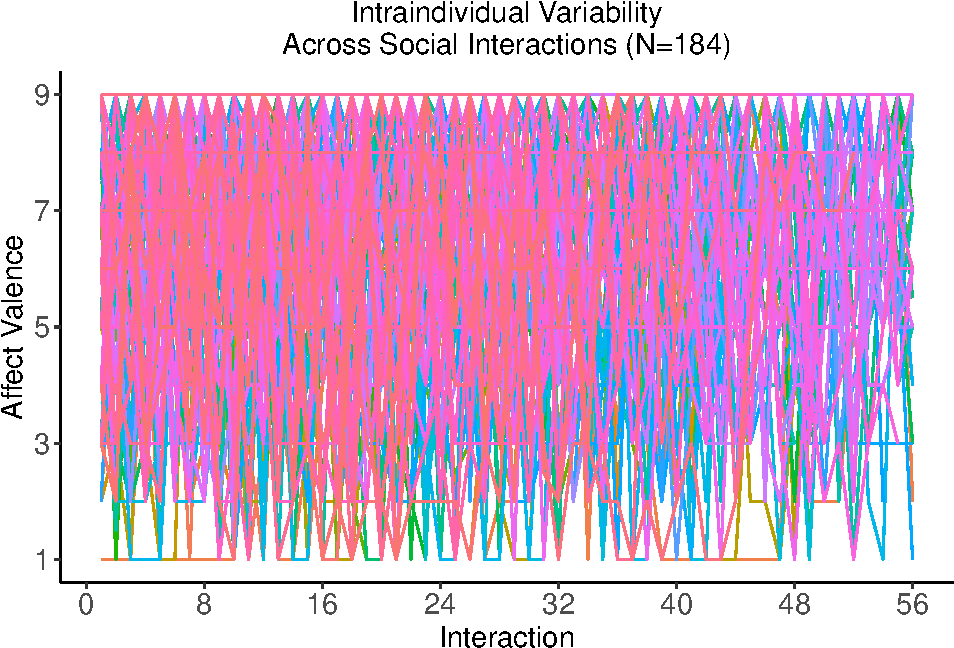
\includegraphics[keepaspectratio]{02_data-descriptives-dataviz_files/figure-latex/plot overtime-1.pdf}}

That ``blob'' is not very informative.
Better to consider a subset of persons or to consider \emph{intraindividual} plots - how each individual person changes over time.

\subsection{Plotting one variable over time for subset of persons}\label{plotting-one-variable-over-time-for-subset-of-persons}

\begin{Shaded}
\begin{Highlighting}[]
\CommentTok{\# plotting intraindividual change }
\NormalTok{interaction\_long }\SpecialCharTok{\%\textgreater{}\%}
  \FunctionTok{filter}\NormalTok{(id }\SpecialCharTok{\textless{}} \DecValTok{112}\NormalTok{) }\SpecialCharTok{\%\textgreater{}\%} \CommentTok{\#filter for ids 101{-}111}
  \FunctionTok{ggplot}\NormalTok{(}\FunctionTok{aes}\NormalTok{(}\AttributeTok{x=}\NormalTok{interaction, }\AttributeTok{group=}\NormalTok{id), }\AttributeTok{color=}\FunctionTok{factor}\NormalTok{(id)) }\SpecialCharTok{+}
  \FunctionTok{guides}\NormalTok{(}\AttributeTok{color=}\StringTok{"none"}\NormalTok{) }\SpecialCharTok{+} \CommentTok{\#to suppress guide}
  \CommentTok{\# first variable}
  \FunctionTok{geom\_line}\NormalTok{(}\FunctionTok{aes}\NormalTok{(}\AttributeTok{y=}\NormalTok{agval, }\AttributeTok{color=}\FunctionTok{factor}\NormalTok{(id))) }\SpecialCharTok{+}
  \CommentTok{\# plot layouts}
  \FunctionTok{scale\_x\_continuous}\NormalTok{(}\AttributeTok{breaks=}\FunctionTok{c}\NormalTok{(}\DecValTok{0}\NormalTok{,}\DecValTok{8}\NormalTok{,}\DecValTok{16}\NormalTok{,}\DecValTok{24}\NormalTok{,}\DecValTok{32}\NormalTok{,}\DecValTok{40}\NormalTok{,}\DecValTok{48}\NormalTok{,}\DecValTok{56}\NormalTok{), }\AttributeTok{name=}\StringTok{"Interaction"}\NormalTok{) }\SpecialCharTok{+}
  \FunctionTok{scale\_y\_continuous}\NormalTok{(}\AttributeTok{breaks=}\FunctionTok{c}\NormalTok{(}\DecValTok{1}\NormalTok{,}\DecValTok{3}\NormalTok{,}\DecValTok{5}\NormalTok{,}\DecValTok{7}\NormalTok{,}\DecValTok{9}\NormalTok{), }\AttributeTok{name=}\StringTok{"Affect Valence"}\NormalTok{) }\SpecialCharTok{+}  
  \FunctionTok{ggtitle}\NormalTok{(}\StringTok{"Intraindividual Variability}\SpecialCharTok{\textbackslash{}n}\StringTok{Across Social Interactions (n=10)"}\NormalTok{) }\SpecialCharTok{+}
  \FunctionTok{theme\_classic}\NormalTok{() }\SpecialCharTok{+}
  \FunctionTok{theme}\NormalTok{(}\AttributeTok{axis.title=}\FunctionTok{element\_text}\NormalTok{(}\AttributeTok{size=}\DecValTok{14}\NormalTok{),}
        \AttributeTok{axis.text=}\FunctionTok{element\_text}\NormalTok{(}\AttributeTok{size=}\DecValTok{14}\NormalTok{),}
        \AttributeTok{plot.title=}\FunctionTok{element\_text}\NormalTok{(}\AttributeTok{size=}\DecValTok{14}\NormalTok{, }\AttributeTok{hjust=}\NormalTok{.}\DecValTok{5}\NormalTok{))}
\end{Highlighting}
\end{Shaded}

\pandocbounded{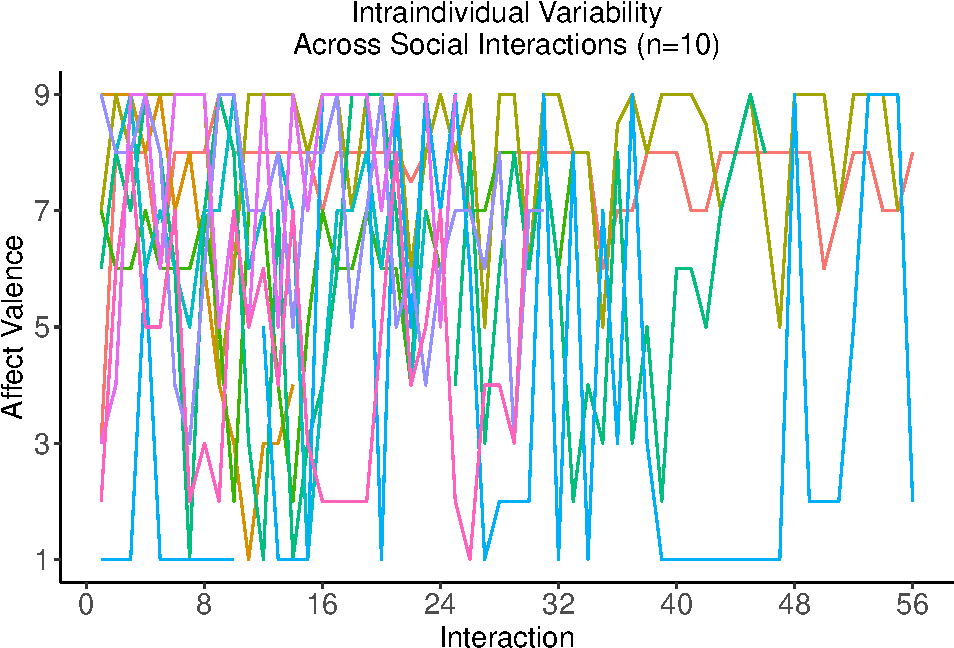
\includegraphics[keepaspectratio]{02_data-descriptives-dataviz_files/figure-latex/plot overtime subset-1.pdf}}

Now move on to \emph{intraindividual} plots

\subsection{Plotting two variables for one person}\label{plotting-two-variables-for-one-person}

\begin{Shaded}
\begin{Highlighting}[]
\CommentTok{\#set colors}
\NormalTok{cols }\OtherTok{\textless{}{-}} \FunctionTok{c}\NormalTok{(}\StringTok{"Affect Valence"}\OtherTok{=}\StringTok{"\#F27781"}\NormalTok{, }\StringTok{"Stress"}\OtherTok{=}\StringTok{"\#18298C"}\NormalTok{)}
\CommentTok{\#plotting intraindividual change }
\NormalTok{interaction\_long }\SpecialCharTok{\%\textgreater{}\%}
  \FunctionTok{filter}\NormalTok{(id }\SpecialCharTok{==} \DecValTok{104}\NormalTok{) }\SpecialCharTok{\%\textgreater{}\%}
  \FunctionTok{ggplot}\NormalTok{(}\FunctionTok{aes}\NormalTok{(}\AttributeTok{x=}\NormalTok{interaction, }\AttributeTok{group=}\NormalTok{ id)) }\SpecialCharTok{+}
  \CommentTok{\# first variable}
  \FunctionTok{geom\_line}\NormalTok{(}\FunctionTok{aes}\NormalTok{(}\AttributeTok{y=}\NormalTok{agval, }\AttributeTok{colour=}\StringTok{"Affect Valence"}\NormalTok{)) }\SpecialCharTok{+}
  \FunctionTok{geom\_point}\NormalTok{(}\FunctionTok{aes}\NormalTok{(}\AttributeTok{y=}\NormalTok{agval, }\AttributeTok{colour=}\StringTok{"Affect Valence"}\NormalTok{)) }\SpecialCharTok{+}
  \CommentTok{\# second variable}
  \FunctionTok{geom\_line}\NormalTok{(}\FunctionTok{aes}\NormalTok{(}\AttributeTok{y=}\NormalTok{stress, }\AttributeTok{color=}\StringTok{"Stress"}\NormalTok{)) }\SpecialCharTok{+}
  \FunctionTok{geom\_point}\NormalTok{(}\FunctionTok{aes}\NormalTok{(}\AttributeTok{y=}\NormalTok{stress, }\AttributeTok{color=}\StringTok{"Stress"}\NormalTok{)) }\SpecialCharTok{+}
  \CommentTok{\# plot layouts}
  \FunctionTok{scale\_x\_continuous}\NormalTok{(}\AttributeTok{breaks=}\FunctionTok{c}\NormalTok{(}\DecValTok{0}\NormalTok{,}\DecValTok{8}\NormalTok{,}\DecValTok{16}\NormalTok{,}\DecValTok{24}\NormalTok{,}\DecValTok{32}\NormalTok{,}\DecValTok{40}\NormalTok{,}\DecValTok{48}\NormalTok{,}\DecValTok{56}\NormalTok{), }\AttributeTok{name=}\StringTok{"Social Interaction"}\NormalTok{) }\SpecialCharTok{+}
  \FunctionTok{scale\_y\_continuous}\NormalTok{(}\AttributeTok{breaks=}\FunctionTok{c}\NormalTok{(}\DecValTok{0}\NormalTok{,}\DecValTok{2}\NormalTok{,}\DecValTok{4}\NormalTok{,}\DecValTok{6}\NormalTok{,}\DecValTok{8}\NormalTok{), }\AttributeTok{name=}\StringTok{"Affect Valence \& Stress"}\NormalTok{) }\SpecialCharTok{+} 
  \FunctionTok{scale\_color\_manual}\NormalTok{(}\AttributeTok{name=}\StringTok{""}\NormalTok{, }\AttributeTok{values =}\NormalTok{ cols) }\SpecialCharTok{+}
  \FunctionTok{ggtitle}\NormalTok{(}\StringTok{"Intraindividual Variability in Affect Valence and Stress}\SpecialCharTok{\textbackslash{}n}\StringTok{Across Social Interactions (n=1)"}\NormalTok{) }\SpecialCharTok{+}
  \FunctionTok{theme\_classic}\NormalTok{() }\SpecialCharTok{+}
  \FunctionTok{theme}\NormalTok{(}\AttributeTok{axis.title=}\FunctionTok{element\_text}\NormalTok{(}\AttributeTok{size=}\DecValTok{14}\NormalTok{),}
        \AttributeTok{axis.text=}\FunctionTok{element\_text}\NormalTok{(}\AttributeTok{size=}\DecValTok{14}\NormalTok{),}
        \AttributeTok{plot.title=}\FunctionTok{element\_text}\NormalTok{(}\AttributeTok{size=}\DecValTok{14}\NormalTok{, }\AttributeTok{hjust=}\NormalTok{.}\DecValTok{5}\NormalTok{),}
        \AttributeTok{legend.text=}\FunctionTok{element\_text}\NormalTok{(}\AttributeTok{size=}\DecValTok{14}\NormalTok{))}
\end{Highlighting}
\end{Shaded}

\pandocbounded{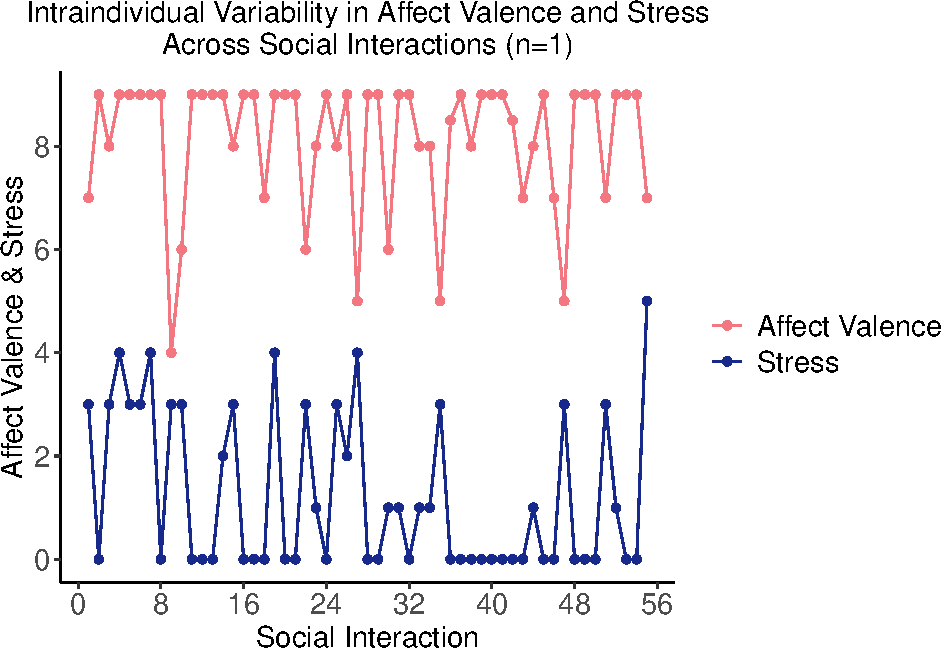
\includegraphics[keepaspectratio]{02_data-descriptives-dataviz_files/figure-latex/plot two vars one person-1.pdf}}

Line plots are good for continuous variables.
Note however, that the scales for these two variables do overlap, but are not exactly the same.

\subsection{Including a categorical variable.}\label{including-a-categorical-variable.}

We can effectively use the background to display categorical variables using the \texttt{geom\_rect()} function within \texttt{ggplot()}.

\subsection{Plotting three variables for one person}\label{plotting-three-variables-for-one-person}

\begin{Shaded}
\begin{Highlighting}[]
\CommentTok{\#set colors}
\NormalTok{cols }\OtherTok{\textless{}{-}} \FunctionTok{c}\NormalTok{(}\StringTok{"Affect Valence"}\OtherTok{=}\StringTok{"\#F27781"}\NormalTok{, }\StringTok{"Stress"}\OtherTok{=}\StringTok{"\#18298C"}\NormalTok{)}
\CommentTok{\#plotting intraindividual change }
\NormalTok{interaction\_long }\SpecialCharTok{\%\textgreater{}\%}
  \FunctionTok{filter}\NormalTok{(id }\SpecialCharTok{==} \DecValTok{104}\NormalTok{) }\SpecialCharTok{\%\textgreater{}\%}
  \FunctionTok{ggplot}\NormalTok{(}\FunctionTok{aes}\NormalTok{(}\AttributeTok{x=}\NormalTok{interaction, }\AttributeTok{group=}\NormalTok{id)) }\SpecialCharTok{+}
  \CommentTok{\#categorical variable as background}
  \FunctionTok{geom\_rect}\NormalTok{(}\FunctionTok{aes}\NormalTok{(}\AttributeTok{xmin=}\NormalTok{interaction}\FloatTok{{-}.5}\NormalTok{, }\AttributeTok{xmax=}\NormalTok{interaction}\FloatTok{+.5}\NormalTok{, }\AttributeTok{ymin=}\DecValTok{0}\NormalTok{, }\AttributeTok{ymax=}\DecValTok{10}\NormalTok{,}
                \AttributeTok{fill=}\FunctionTok{factor}\NormalTok{(partner\_gender)), }\AttributeTok{alpha=}\FloatTok{0.2}\NormalTok{) }\SpecialCharTok{+}
  \CommentTok{\# first variable}
  \FunctionTok{geom\_line}\NormalTok{(}\FunctionTok{aes}\NormalTok{(}\AttributeTok{y=}\NormalTok{agval, }\AttributeTok{colour=}\StringTok{"Affect Valence"}\NormalTok{)) }\SpecialCharTok{+}
  \FunctionTok{geom\_point}\NormalTok{(}\FunctionTok{aes}\NormalTok{(}\AttributeTok{y=}\NormalTok{agval, }\AttributeTok{colour=}\StringTok{"Affect Valence"}\NormalTok{)) }\SpecialCharTok{+}
  \CommentTok{\# second variable}
  \FunctionTok{geom\_line}\NormalTok{(}\FunctionTok{aes}\NormalTok{(}\AttributeTok{y=}\NormalTok{stress, }\AttributeTok{color=}\StringTok{"Stress"}\NormalTok{)) }\SpecialCharTok{+}
  \FunctionTok{geom\_point}\NormalTok{(}\FunctionTok{aes}\NormalTok{(}\AttributeTok{y=}\NormalTok{stress, }\AttributeTok{color=}\StringTok{"Stress"}\NormalTok{)) }\SpecialCharTok{+}
  \CommentTok{\# plot layouts}
  \FunctionTok{scale\_color\_manual}\NormalTok{(}\AttributeTok{name=}\StringTok{""}\NormalTok{, }\AttributeTok{values =}\NormalTok{ cols) }\SpecialCharTok{+}
  \FunctionTok{scale\_fill\_manual}\NormalTok{(}\AttributeTok{name =} \StringTok{"Partner Gender"}\NormalTok{,}
                    \AttributeTok{values =} \FunctionTok{c}\NormalTok{(}\StringTok{"\#F29E03"}\NormalTok{, }\StringTok{"\#20BDA1"}\NormalTok{), }
                    \AttributeTok{labels =} \FunctionTok{c}\NormalTok{(}\StringTok{"female"}\NormalTok{, }\StringTok{"male"}\NormalTok{, }\StringTok{"missing"}\NormalTok{),}
                    \AttributeTok{na.value=}\StringTok{"black"}\NormalTok{) }\SpecialCharTok{+} 
  \FunctionTok{scale\_x\_continuous}\NormalTok{(}\AttributeTok{breaks=}\FunctionTok{c}\NormalTok{(}\DecValTok{0}\NormalTok{,}\DecValTok{8}\NormalTok{,}\DecValTok{16}\NormalTok{,}\DecValTok{24}\NormalTok{,}\DecValTok{32}\NormalTok{,}\DecValTok{40}\NormalTok{,}\DecValTok{48}\NormalTok{,}\DecValTok{56}\NormalTok{), }\AttributeTok{name=}\StringTok{"Social Interaction"}\NormalTok{) }\SpecialCharTok{+}
  \FunctionTok{scale\_y\_continuous}\NormalTok{(}\AttributeTok{breaks=}\FunctionTok{c}\NormalTok{(}\DecValTok{0}\NormalTok{,}\DecValTok{2}\NormalTok{,}\DecValTok{4}\NormalTok{,}\DecValTok{6}\NormalTok{,}\DecValTok{8}\NormalTok{), }\AttributeTok{name=}\StringTok{"Affect Valence \& Stress"}\NormalTok{) }\SpecialCharTok{+} 
  \FunctionTok{ggtitle}\NormalTok{(}\StringTok{"Intraindividual Variability in Affect Valence and Stress}\SpecialCharTok{\textbackslash{}n}\StringTok{Across Social Interactions with Male and Female Partners (n=1)"}\NormalTok{) }\SpecialCharTok{+}
  \FunctionTok{theme\_classic}\NormalTok{() }\SpecialCharTok{+}
  \FunctionTok{theme}\NormalTok{(}\AttributeTok{axis.title=}\FunctionTok{element\_text}\NormalTok{(}\AttributeTok{size=}\DecValTok{14}\NormalTok{),}
        \AttributeTok{axis.text=}\FunctionTok{element\_text}\NormalTok{(}\AttributeTok{size=}\DecValTok{14}\NormalTok{),}
        \AttributeTok{plot.title=}\FunctionTok{element\_text}\NormalTok{(}\AttributeTok{size=}\DecValTok{14}\NormalTok{, }\AttributeTok{hjust=}\NormalTok{.}\DecValTok{5}\NormalTok{))}
\end{Highlighting}
\end{Shaded}

\pandocbounded{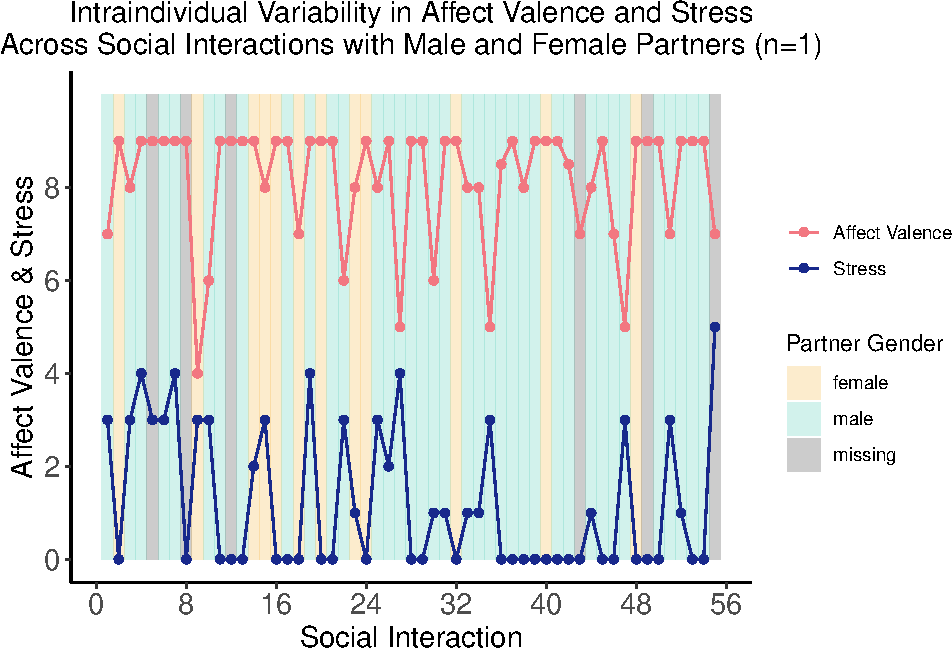
\includegraphics[keepaspectratio]{02_data-descriptives-dataviz_files/figure-latex/plot three vars-1.pdf}}

\subsection{Plotting multiple individuals}\label{plotting-multiple-individuals}

Of course, we are also interested in interindividual differences.
To examine those, we can display multiple persons in separate panels using \texttt{facet\_wrap()}.

\begin{Shaded}
\begin{Highlighting}[]
\CommentTok{\# plotting intraindividual change }
\NormalTok{interaction\_long }\SpecialCharTok{\%\textgreater{}\%}
  \FunctionTok{filter}\NormalTok{(id }\SpecialCharTok{\textless{}=} \DecValTok{106}\NormalTok{) }\SpecialCharTok{\%\textgreater{}\%}
  \FunctionTok{ggplot}\NormalTok{(}\FunctionTok{aes}\NormalTok{(}\AttributeTok{x =}\NormalTok{ interaction, }\AttributeTok{group=} \FunctionTok{factor}\NormalTok{(id))) }\SpecialCharTok{+}
  \FunctionTok{geom\_line}\NormalTok{(}\FunctionTok{aes}\NormalTok{(}\AttributeTok{y=}\NormalTok{agval), }\AttributeTok{colour=}\StringTok{"\#F27781"}\NormalTok{) }\SpecialCharTok{+}
  \FunctionTok{geom\_point}\NormalTok{(}\FunctionTok{aes}\NormalTok{(}\AttributeTok{y=}\NormalTok{agval), }\AttributeTok{colour=}\StringTok{"\#F27781"}\NormalTok{) }\SpecialCharTok{+}
  \FunctionTok{scale\_x\_continuous}\NormalTok{(}\AttributeTok{breaks=}\FunctionTok{c}\NormalTok{(}\DecValTok{0}\NormalTok{,}\DecValTok{8}\NormalTok{,}\DecValTok{16}\NormalTok{,}\DecValTok{24}\NormalTok{,}\DecValTok{32}\NormalTok{,}\DecValTok{40}\NormalTok{,}\DecValTok{48}\NormalTok{,}\DecValTok{56}\NormalTok{), }\AttributeTok{name=}\StringTok{"Social Interaction"}\NormalTok{) }\SpecialCharTok{+}
  \FunctionTok{scale\_y\_continuous}\NormalTok{(}\AttributeTok{breaks=}\FunctionTok{c}\NormalTok{(}\DecValTok{1}\NormalTok{,}\DecValTok{3}\NormalTok{,}\DecValTok{5}\NormalTok{,}\DecValTok{7}\NormalTok{,}\DecValTok{9}\NormalTok{), }\AttributeTok{name=}\StringTok{"Affect Valence"}\NormalTok{) }\SpecialCharTok{+} 
  \FunctionTok{ggtitle}\NormalTok{(}\StringTok{"Intraindividual Variability in Affect Valence}\SpecialCharTok{\textbackslash{}n}\StringTok{Across Social Interactions (n=5)"}\NormalTok{) }\SpecialCharTok{+}
  \FunctionTok{theme\_classic}\NormalTok{() }\SpecialCharTok{+}
  \FunctionTok{theme}\NormalTok{(}\AttributeTok{axis.title=}\FunctionTok{element\_text}\NormalTok{(}\AttributeTok{size=}\DecValTok{14}\NormalTok{),}
        \AttributeTok{axis.text=}\FunctionTok{element\_text}\NormalTok{(}\AttributeTok{size=}\DecValTok{14}\NormalTok{),}
        \AttributeTok{plot.title=}\FunctionTok{element\_text}\NormalTok{(}\AttributeTok{size=}\DecValTok{14}\NormalTok{, }\AttributeTok{hjust=}\NormalTok{.}\DecValTok{5}\NormalTok{)) }\SpecialCharTok{+}
  \FunctionTok{facet\_wrap}\NormalTok{(}\SpecialCharTok{\textasciitilde{}}\NormalTok{id, }\AttributeTok{nrow=}\DecValTok{5}\NormalTok{)}
\end{Highlighting}
\end{Shaded}

\pandocbounded{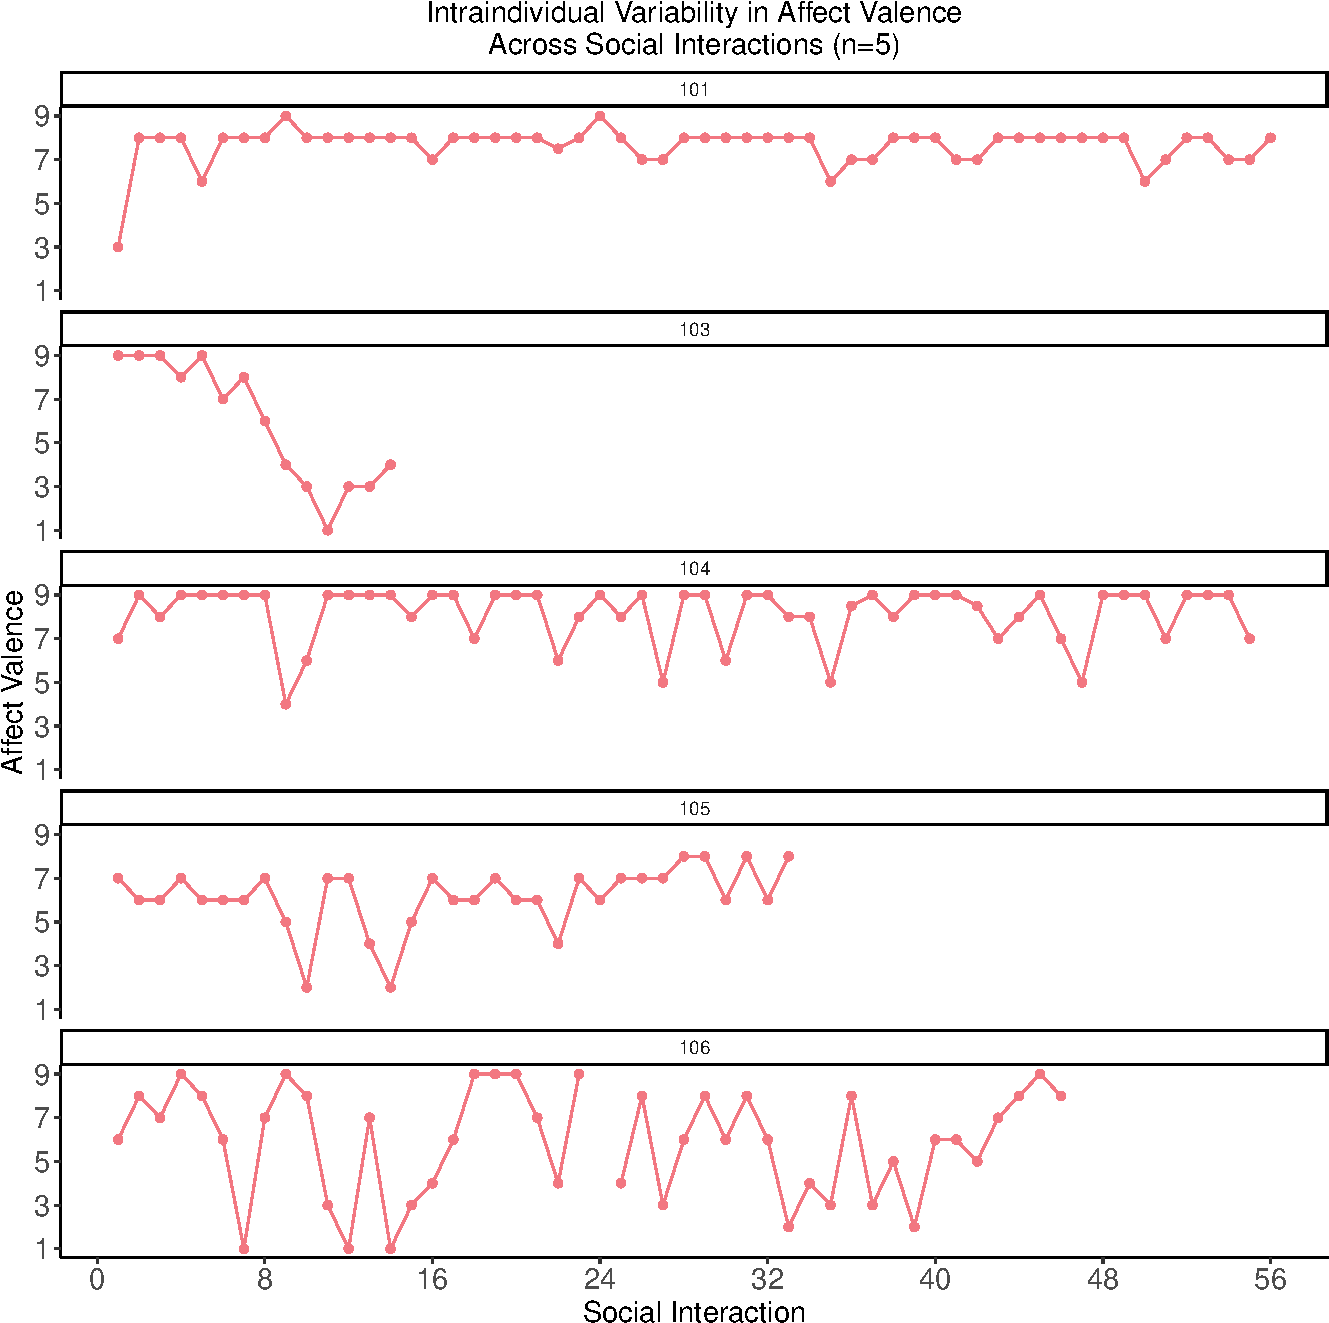
\includegraphics[keepaspectratio]{02_data-descriptives-dataviz_files/figure-latex/plot multiple people-1.pdf}}

\begin{Shaded}
\begin{Highlighting}[]
\CommentTok{\#set colors}
\NormalTok{cols }\OtherTok{\textless{}{-}} \FunctionTok{c}\NormalTok{(}\StringTok{"Affect Valence"}\OtherTok{=}\StringTok{"\#F27781"}\NormalTok{, }\StringTok{"Stress"}\OtherTok{=}\StringTok{"\#18298C"}\NormalTok{)}
\CommentTok{\#plotting intraindividual change }
\NormalTok{interaction\_long }\SpecialCharTok{\%\textgreater{}\%}
  \FunctionTok{filter}\NormalTok{(id }\SpecialCharTok{\textless{}=} \DecValTok{106}\NormalTok{) }\SpecialCharTok{\%\textgreater{}\%}
  \FunctionTok{ggplot}\NormalTok{(}\FunctionTok{aes}\NormalTok{(}\AttributeTok{x =}\NormalTok{ interaction, }\AttributeTok{group=} \FunctionTok{factor}\NormalTok{(id))) }\SpecialCharTok{+}
  \FunctionTok{geom\_line}\NormalTok{(}\FunctionTok{aes}\NormalTok{(}\AttributeTok{y=}\NormalTok{agval, }\AttributeTok{colour=}\StringTok{"Affect Valence"}\NormalTok{)) }\SpecialCharTok{+}
  \FunctionTok{geom\_point}\NormalTok{(}\FunctionTok{aes}\NormalTok{(}\AttributeTok{y=}\NormalTok{agval, }\AttributeTok{colour=}\StringTok{"Affect Valence"}\NormalTok{)) }\SpecialCharTok{+}
  \FunctionTok{geom\_line}\NormalTok{(}\FunctionTok{aes}\NormalTok{(}\AttributeTok{y=}\NormalTok{stress, }\AttributeTok{color=}\StringTok{"Stress"}\NormalTok{)) }\SpecialCharTok{+}
  \FunctionTok{geom\_point}\NormalTok{(}\FunctionTok{aes}\NormalTok{(}\AttributeTok{y=}\NormalTok{stress, }\AttributeTok{color=}\StringTok{"Stress"}\NormalTok{)) }\SpecialCharTok{+}
  \FunctionTok{scale\_x\_continuous}\NormalTok{(}\AttributeTok{breaks=}\FunctionTok{c}\NormalTok{(}\DecValTok{0}\NormalTok{,}\DecValTok{8}\NormalTok{,}\DecValTok{16}\NormalTok{,}\DecValTok{24}\NormalTok{,}\DecValTok{32}\NormalTok{,}\DecValTok{40}\NormalTok{,}\DecValTok{48}\NormalTok{,}\DecValTok{56}\NormalTok{), }\AttributeTok{name=}\StringTok{"Social Interaction"}\NormalTok{) }\SpecialCharTok{+}
  \FunctionTok{scale\_y\_continuous}\NormalTok{(}\AttributeTok{breaks=}\FunctionTok{c}\NormalTok{(}\DecValTok{0}\NormalTok{,}\DecValTok{4}\NormalTok{,}\DecValTok{8}\NormalTok{), }\AttributeTok{name=}\StringTok{"Affect Valence \& Stress"}\NormalTok{) }\SpecialCharTok{+} 
  \FunctionTok{scale\_color\_manual}\NormalTok{(}\AttributeTok{name=}\StringTok{""}\NormalTok{, }\AttributeTok{values =}\NormalTok{ cols) }\SpecialCharTok{+}
  \FunctionTok{ggtitle}\NormalTok{(}\StringTok{"Intraindividual Variability in Affect Valence and Stress}\SpecialCharTok{\textbackslash{}n}\StringTok{Across Social Interactions (n=5)"}\NormalTok{) }\SpecialCharTok{+}
  \FunctionTok{theme\_classic}\NormalTok{() }\SpecialCharTok{+}
  \FunctionTok{theme}\NormalTok{(}\AttributeTok{axis.title=}\FunctionTok{element\_text}\NormalTok{(}\AttributeTok{size=}\DecValTok{14}\NormalTok{),}
        \AttributeTok{axis.text=}\FunctionTok{element\_text}\NormalTok{(}\AttributeTok{size=}\DecValTok{14}\NormalTok{),}
        \AttributeTok{plot.title=}\FunctionTok{element\_text}\NormalTok{(}\AttributeTok{size=}\DecValTok{14}\NormalTok{, }\AttributeTok{hjust=}\NormalTok{.}\DecValTok{5}\NormalTok{),}
        \AttributeTok{legend.text=}\FunctionTok{element\_text}\NormalTok{(}\AttributeTok{size=}\DecValTok{14}\NormalTok{)) }\SpecialCharTok{+}
  \FunctionTok{facet\_wrap}\NormalTok{(}\SpecialCharTok{\textasciitilde{}}\NormalTok{id, }\AttributeTok{nrow=}\DecValTok{5}\NormalTok{)}
\end{Highlighting}
\end{Shaded}

\pandocbounded{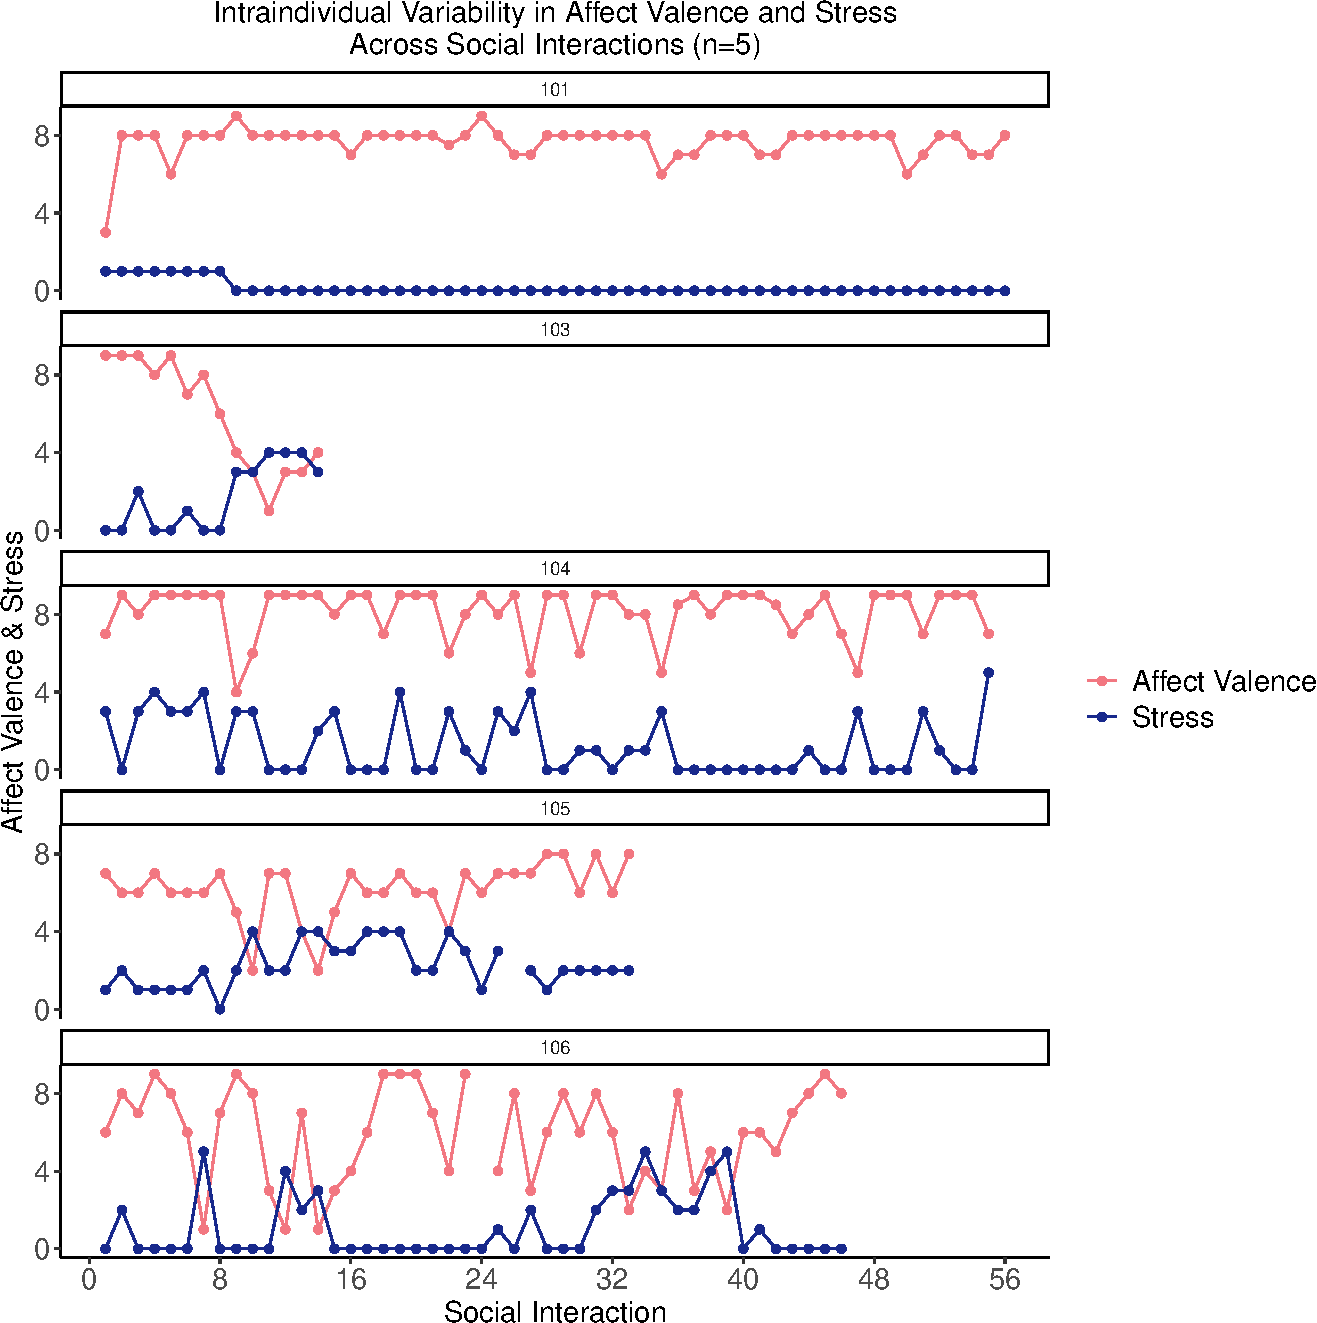
\includegraphics[keepaspectratio]{02_data-descriptives-dataviz_files/figure-latex/plot multiple 2-1.pdf}}

\begin{Shaded}
\begin{Highlighting}[]
\CommentTok{\#set colors}
\NormalTok{cols }\OtherTok{\textless{}{-}} \FunctionTok{c}\NormalTok{(}\StringTok{"Affect Valence"}\OtherTok{=}\StringTok{"\#F27781"}\NormalTok{, }\StringTok{"Stress"}\OtherTok{=}\StringTok{"\#18298C"}\NormalTok{)}
\CommentTok{\#plotting intraindividual change }
\NormalTok{interaction\_long }\SpecialCharTok{\%\textgreater{}\%}
  \FunctionTok{filter}\NormalTok{(id }\SpecialCharTok{\textless{}=} \DecValTok{106}\NormalTok{) }\SpecialCharTok{\%\textgreater{}\%}
  \FunctionTok{ggplot}\NormalTok{(}\FunctionTok{aes}\NormalTok{(}\AttributeTok{x =}\NormalTok{ interaction, }\AttributeTok{group=} \FunctionTok{factor}\NormalTok{(id))) }\SpecialCharTok{+}
  \CommentTok{\#categorical variable as background}
  \FunctionTok{geom\_rect}\NormalTok{(}\FunctionTok{aes}\NormalTok{(}\AttributeTok{xmin=}\NormalTok{interaction}\FloatTok{{-}.5}\NormalTok{, }\AttributeTok{xmax=}\NormalTok{interaction}\FloatTok{+.5}\NormalTok{, }\AttributeTok{ymin=}\DecValTok{0}\NormalTok{, }\AttributeTok{ymax=}\DecValTok{9}\NormalTok{,}
                \AttributeTok{fill=}\FunctionTok{factor}\NormalTok{(partner\_gender)), }\AttributeTok{alpha=}\FloatTok{0.2}\NormalTok{) }\SpecialCharTok{+}
  \CommentTok{\#first variable}
  \FunctionTok{geom\_line}\NormalTok{(}\FunctionTok{aes}\NormalTok{(}\AttributeTok{y=}\NormalTok{agval, }\AttributeTok{colour=}\StringTok{"Affect Valence"}\NormalTok{)) }\SpecialCharTok{+}
  \FunctionTok{geom\_point}\NormalTok{(}\FunctionTok{aes}\NormalTok{(}\AttributeTok{y=}\NormalTok{agval, }\AttributeTok{colour=}\StringTok{"Affect Valence"}\NormalTok{)) }\SpecialCharTok{+}
  \CommentTok{\#second variable}
  \FunctionTok{geom\_line}\NormalTok{(}\FunctionTok{aes}\NormalTok{(}\AttributeTok{y=}\NormalTok{stress, }\AttributeTok{color=}\StringTok{"Stress"}\NormalTok{)) }\SpecialCharTok{+}
  \FunctionTok{geom\_point}\NormalTok{(}\FunctionTok{aes}\NormalTok{(}\AttributeTok{y=}\NormalTok{stress, }\AttributeTok{color=}\StringTok{"Stress"}\NormalTok{)) }\SpecialCharTok{+}
  \CommentTok{\#plot layouts}
  \FunctionTok{scale\_color\_manual}\NormalTok{(}\AttributeTok{name=}\StringTok{""}\NormalTok{, }\AttributeTok{values =}\NormalTok{ cols) }\SpecialCharTok{+}
  \FunctionTok{scale\_fill\_manual}\NormalTok{(}\AttributeTok{name =} \StringTok{"Partner Gender"}\NormalTok{,}
                    \AttributeTok{values =} \FunctionTok{c}\NormalTok{(}\StringTok{"\#F29E03"}\NormalTok{, }\StringTok{"\#20BDA1"}\NormalTok{), }
                    \AttributeTok{labels =} \FunctionTok{c}\NormalTok{(}\StringTok{"female"}\NormalTok{, }\StringTok{"male"}\NormalTok{, }\StringTok{"missing"}\NormalTok{),}
                    \AttributeTok{na.value=}\StringTok{"black"}\NormalTok{) }\SpecialCharTok{+} 
  \FunctionTok{scale\_x\_continuous}\NormalTok{(}\AttributeTok{breaks=}\FunctionTok{c}\NormalTok{(}\DecValTok{0}\NormalTok{,}\DecValTok{8}\NormalTok{,}\DecValTok{16}\NormalTok{,}\DecValTok{24}\NormalTok{,}\DecValTok{32}\NormalTok{,}\DecValTok{40}\NormalTok{,}\DecValTok{48}\NormalTok{,}\DecValTok{56}\NormalTok{), }\AttributeTok{name=}\StringTok{"Social Interaction"}\NormalTok{) }\SpecialCharTok{+}
  \FunctionTok{scale\_y\_continuous}\NormalTok{(}\AttributeTok{breaks=}\FunctionTok{c}\NormalTok{(}\DecValTok{0}\NormalTok{,}\DecValTok{2}\NormalTok{,}\DecValTok{4}\NormalTok{,}\DecValTok{6}\NormalTok{,}\DecValTok{8}\NormalTok{), }\AttributeTok{name=}\StringTok{"Affect Valence \& Stress"}\NormalTok{) }\SpecialCharTok{+}  
  \FunctionTok{ggtitle}\NormalTok{(}\StringTok{"Intraindividual Variability in Affect Valence and Stress}\SpecialCharTok{\textbackslash{}n}\StringTok{Across Social Interactions with Male and Female Partners (n=1)"}\NormalTok{) }\SpecialCharTok{+}
  \FunctionTok{theme\_classic}\NormalTok{() }\SpecialCharTok{+}
  \FunctionTok{theme}\NormalTok{(}\AttributeTok{axis.title=}\FunctionTok{element\_text}\NormalTok{(}\AttributeTok{size=}\DecValTok{14}\NormalTok{),}
        \AttributeTok{axis.text=}\FunctionTok{element\_text}\NormalTok{(}\AttributeTok{size=}\DecValTok{14}\NormalTok{),}
        \AttributeTok{plot.title=}\FunctionTok{element\_text}\NormalTok{(}\AttributeTok{size=}\DecValTok{14}\NormalTok{, }\AttributeTok{hjust=}\NormalTok{.}\DecValTok{5}\NormalTok{)) }\SpecialCharTok{+}
  \FunctionTok{facet\_wrap}\NormalTok{(}\SpecialCharTok{\textasciitilde{}}\NormalTok{id, }\AttributeTok{nrow=}\DecValTok{5}\NormalTok{)}
\end{Highlighting}
\end{Shaded}

\pandocbounded{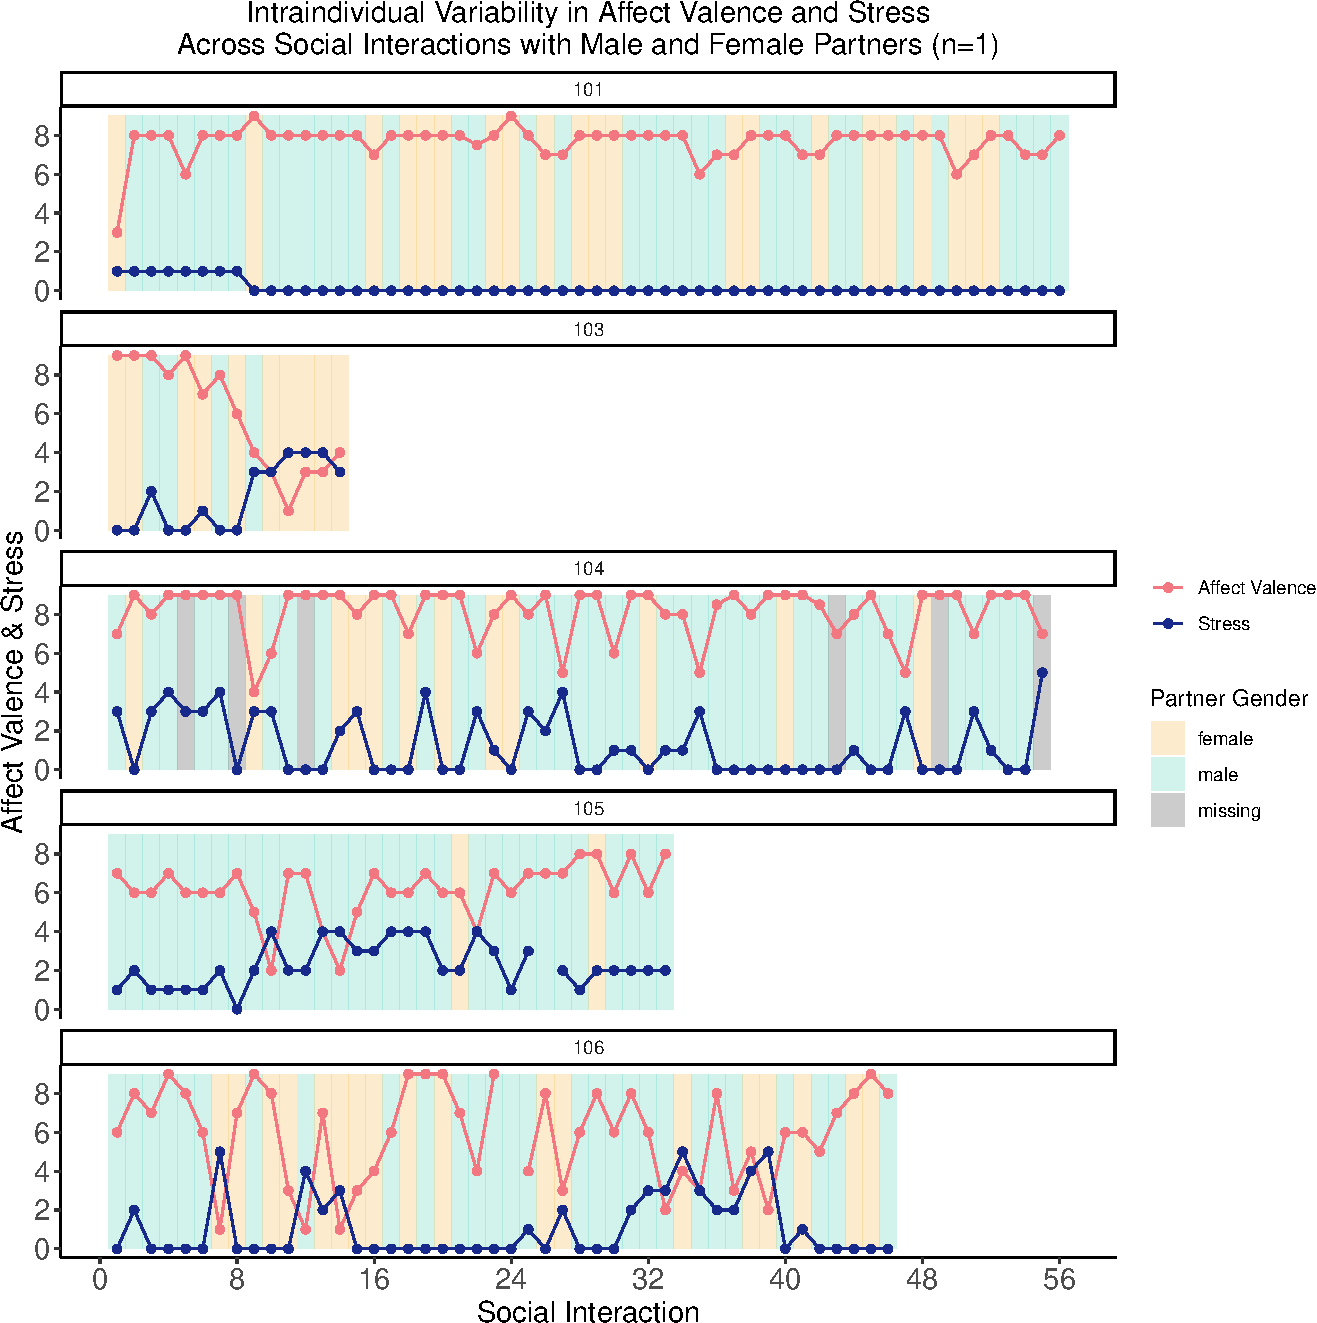
\includegraphics[keepaspectratio]{02_data-descriptives-dataviz_files/figure-latex/plot3-1.pdf}}

\section{Conclusion}\label{conclusion}

This tutorial covered some basics, including reading in repeated measures data from an experience sampling study, manipulating those data into two different structures (long and wide), assessing the overall characteristics of the data/protocol, and describing the data (descriptives and plots).

We hope this foundational material prompts development of some general strategies that can be applied whenever approaching new longitudinal data.
The best part is that, after looking at the above plots, we know that subsequent analyses will be super fun!

\textbf{Thanks for playing!}

\section{Captioned figures and tables}\label{captioned-figures-and-tables}

Figures and tables \emph{with captions} can also be cross-referenced from elsewhere in your book using \texttt{\textbackslash{}@ref(fig:chunk-label)} and \texttt{\textbackslash{}@ref(tab:chunk-label)}, respectively.

See Figure \ref{fig:nice-fig}.

\begin{Shaded}
\begin{Highlighting}[]
\FunctionTok{par}\NormalTok{(}\AttributeTok{mar =} \FunctionTok{c}\NormalTok{(}\DecValTok{4}\NormalTok{, }\DecValTok{4}\NormalTok{, .}\DecValTok{1}\NormalTok{, .}\DecValTok{1}\NormalTok{))}
\FunctionTok{plot}\NormalTok{(pressure, }\AttributeTok{type =} \StringTok{\textquotesingle{}b\textquotesingle{}}\NormalTok{, }\AttributeTok{pch =} \DecValTok{19}\NormalTok{)}
\end{Highlighting}
\end{Shaded}

\begin{figure}

{\centering 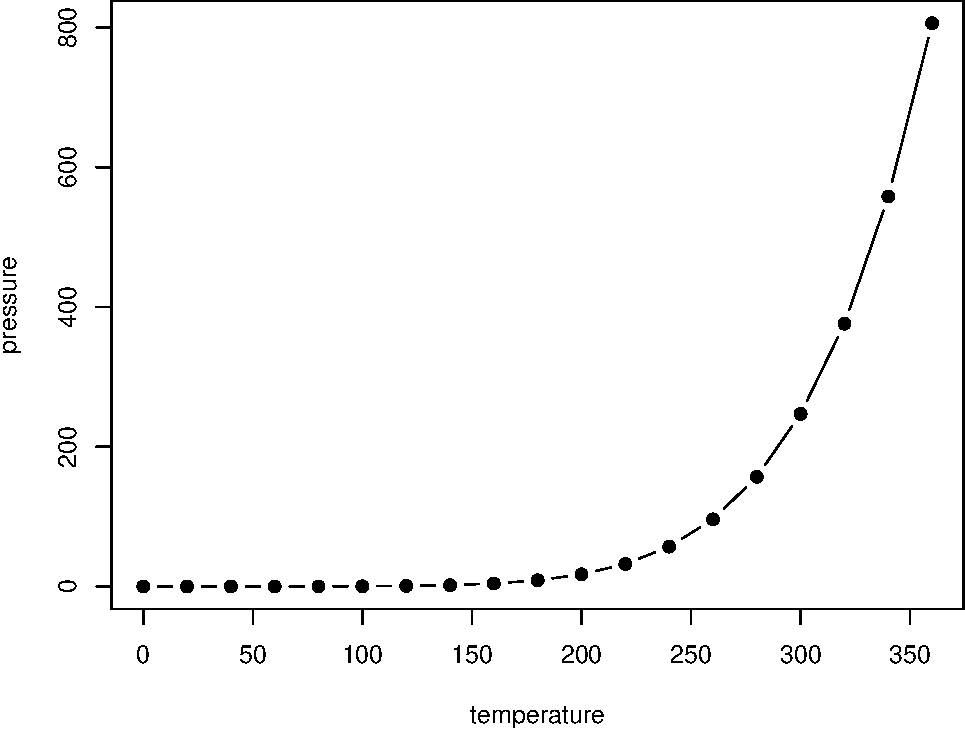
\includegraphics[width=0.8\linewidth,alt={Plot with connected points showing that vapor pressure of mercury increases exponentially as temperature increases.}]{02_data-descriptives-dataviz_files/figure-latex/nice-fig-1} 

}

\caption{Here is a nice figure!}\label{fig:nice-fig}
\end{figure}

Don't miss Table \ref{tab:nice-tab}.

\begin{Shaded}
\begin{Highlighting}[]
\NormalTok{knitr}\SpecialCharTok{::}\FunctionTok{kable}\NormalTok{(}
  \FunctionTok{head}\NormalTok{(pressure, }\DecValTok{10}\NormalTok{), }\AttributeTok{caption =} \StringTok{\textquotesingle{}Here is a nice table!\textquotesingle{}}\NormalTok{,}
  \AttributeTok{booktabs =} \ConstantTok{TRUE}
\NormalTok{)}
\end{Highlighting}
\end{Shaded}

\begin{table}

\caption{\label{tab:nice-tab}Here is a nice table!}
\centering
\begin{tabular}[t]{rr}
\toprule
temperature & pressure\\
\midrule
0 & 0.0002\\
20 & 0.0012\\
40 & 0.0060\\
60 & 0.0300\\
80 & 0.0900\\
\addlinespace
100 & 0.2700\\
120 & 0.7500\\
140 & 1.8500\\
160 & 4.2000\\
180 & 8.8000\\
\bottomrule
\end{tabular}
\end{table}

\chapter{Parts}\label{parts}

You can add parts to organize one or more book chapters together. Parts can be inserted at the top of an .Rmd file, before the first-level chapter heading in that same file.

Add a numbered part: \texttt{\#\ (PART)\ Act\ one\ \{-\}} (followed by \texttt{\#\ A\ chapter})

Add an unnumbered part: \texttt{\#\ (PART\textbackslash{}*)\ Act\ one\ \{-\}} (followed by \texttt{\#\ A\ chapter})

Add an appendix as a special kind of un-numbered part: \texttt{\#\ (APPENDIX)\ Other\ stuff\ \{-\}} (followed by \texttt{\#\ A\ chapter}). Chapters in an appendix are prepended with letters instead of numbers.

\chapter{Footnotes and citations}\label{footnotes-and-citations}

\section{Footnotes}\label{footnotes}

Footnotes are put inside the square brackets after a caret \texttt{\^{}{[}{]}}. Like this one \footnote{This is a footnote.}.

\section{Citations}\label{citations}

Reference items in your bibliography file(s) using \texttt{@key}.

\citet{burkner_brms_2017}
\citet{wickham_dplyr_2023}

For example, we are using the \textbf{bookdown} package \citep{R-bookdown} (check out the last code chunk in index.Rmd to see how this citation key was added) in this sample book, which was built on top of R Markdown and \textbf{knitr} \citep{xie2015} (this citation was added manually in an external file book.bib).
Note that the \texttt{.bib} files need to be listed in the index.Rmd with the YAML \texttt{bibliography} key.

The \texttt{bs4\_book} theme makes footnotes appear inline when you click on them. In this example book, we added \texttt{csl:\ chicago-fullnote-bibliography.csl} to the \texttt{index.Rmd} YAML, and include the \texttt{.csl} file. To download a new style, we recommend: \url{https://www.zotero.org/styles/}

The RStudio Visual Markdown Editor can also make it easier to insert citations: \url{https://rstudio.github.io/visual-markdown-editing/\#/citations}

\chapter{Blocks}\label{blocks}

\section{Equations}\label{equations}

Here is an equation.

\begin{equation} 
  f\left(k\right) = \binom{n}{k} p^k\left(1-p\right)^{n-k}
  \label{eq:binom}
\end{equation}

You may refer to using \texttt{\textbackslash{}@ref(eq:binom)}, like see Equation \eqref{eq:binom}.

\section{Theorems and proofs}\label{theorems-and-proofs}

Labeled theorems can be referenced in text using \texttt{\textbackslash{}@ref(thm:tri)}, for example, check out this smart theorem \ref{thm:tri}.

\begin{theorem}
\protect\hypertarget{thm:tri}{}\label{thm:tri}For a right triangle, if \(c\) denotes the \emph{length} of the hypotenuse
and \(a\) and \(b\) denote the lengths of the \textbf{other} two sides, we have
\[a^2 + b^2 = c^2\]
\end{theorem}

Read more here \url{https://bookdown.org/yihui/bookdown/markdown-extensions-by-bookdown.html}.

\section{Callout blocks}\label{callout-blocks}

The \texttt{bs4\_book} theme also includes special callout blocks, like this \texttt{.rmdnote}.

You can use \textbf{markdown} inside a block.

\begin{Shaded}
\begin{Highlighting}[]
\FunctionTok{head}\NormalTok{(beaver1, }\AttributeTok{n =} \DecValTok{5}\NormalTok{)}
\CommentTok{\#\textgreater{}   day time  temp activ}
\CommentTok{\#\textgreater{} 1 346  840 36.33     0}
\CommentTok{\#\textgreater{} 2 346  850 36.34     0}
\CommentTok{\#\textgreater{} 3 346  900 36.35     0}
\CommentTok{\#\textgreater{} 4 346  910 36.42     0}
\CommentTok{\#\textgreater{} 5 346  920 36.55     0}
\end{Highlighting}
\end{Shaded}

It is up to the user to define the appearance of these blocks for LaTeX output.

You may also use: \texttt{.rmdcaution}, \texttt{.rmdimportant}, \texttt{.rmdtip}, or \texttt{.rmdwarning} as the block name.

The R Markdown Cookbook provides more help on how to use custom blocks to design your own callouts: \url{https://bookdown.org/yihui/rmarkdown-cookbook/custom-blocks.html}

\chapter{Sharing your book}\label{sharing-your-book}

\section{Publishing}\label{publishing}

HTML books can be published online, see: \url{https://bookdown.org/yihui/bookdown/publishing.html}

\section{404 pages}\label{pages}

By default, users will be directed to a 404 page if they try to access a webpage that cannot be found. If you'd like to customize your 404 page instead of using the default, you may add either a \texttt{\_404.Rmd} or \texttt{\_404.md} file to your project root and use code and/or Markdown syntax.

\section{Metadata for sharing}\label{metadata-for-sharing}

Bookdown HTML books will provide HTML metadata for social sharing on platforms like Twitter, Facebook, and LinkedIn, using information you provide in the \texttt{index.Rmd} YAML. To setup, set the \texttt{url} for your book and the path to your \texttt{cover-image} file. Your book's \texttt{title} and \texttt{description} are also used.

This \texttt{bs4\_book} provides enhanced metadata for social sharing, so that each chapter shared will have a unique description, auto-generated based on the content.

Specify your book's source repository on GitHub as the \texttt{repo} in the \texttt{\_output.yml} file, which allows users to view each chapter's source file or suggest an edit. Read more about the features of this output format here:

\url{https://pkgs.rstudio.com/bookdown/reference/bs4_book.html}

Or use:

\begin{Shaded}
\begin{Highlighting}[]
\NormalTok{?bookdown}\SpecialCharTok{::}\NormalTok{bs4\_book}
\end{Highlighting}
\end{Shaded}


  \bibliography{R\_Tutorials.bib,packages.bib}

\end{document}
